%%% Local Variables: 
%%% coding: utf-8
%%% mode: latex
%%% TeX-engine: xetex
%%% End: 

\documentclass[hide notes,intlimits]{beamer}

\mode<presentation>
{
  \usetheme{UAFshade}
  \setbeamercovered{transparent}
}

% load packages
\usepackage{media9}
\usepackage[english]{babel}
\usepackage{lmodern}
\usepackage[multidot]{grffile}
\usepackage{tikz}
\usetikzlibrary{shadows}

% \usepackage{pgfpages}
% \setbeamertemplate{note page}[plain]
% \setbeameroption{show notes on second screen=right}


\definecolor{dark red}{HTML}{E41A1C}
\definecolor{dark green}{HTML}{4DAF4A}
\definecolor{dark violet}{HTML}{984EA3}
\definecolor{dark blue}{HTML}{084594}
\definecolor{dark orange}{HTML}{FF7F00}
\definecolor{white}{HTML}{FFFFFF}
\definecolor{light blue}{HTML}{377EB8}
\definecolor{light red}{HTML}{FB9A99}
\definecolor{light violet}{HTML}{CAB2D6}

\definecolor{uaf red}{HTML}{E41A1C}
\definecolor{uaf blue}{HTML}{377EB8}
\definecolor{uaf green}{HTML}{4DAF4A}
\definecolor{uaf violet}{HTML}{984EA3}
\definecolor{uaf orange}{HTML}{FF7F00}
\setbeamercolor{boxed}{fg=black,bg=uaf yellow}


\graphicspath{{../figures_2018_08/}{../figures/}}

\setbeamerfont{caption}{size=\scriptsize}

% code adapted from http://tex.stackexchange.com/a/11483/3954

% some parameters for customization
\def\shadowshift{3pt,-3pt}
\def\shadowradius{6pt}

\colorlet{innercolor}{black!60}
\colorlet{outercolor}{gray!05}

% this draws a shadow under a rectangle node
\newcommand\drawshadow[1]{
    \begin{pgfonlayer}{shadow}
        \shade[outercolor,inner color=innercolor,outer color=outercolor] ($(#1.south west)+(\shadowshift)+(\shadowradius/2,\shadowradius/2)$) circle (\shadowradius);
        \shade[outercolor,inner color=innercolor,outer color=outercolor] ($(#1.north west)+(\shadowshift)+(\shadowradius/2,-\shadowradius/2)$) circle (\shadowradius);
        \shade[outercolor,inner color=innercolor,outer color=outercolor] ($(#1.south east)+(\shadowshift)+(-\shadowradius/2,\shadowradius/2)$) circle (\shadowradius);
        \shade[outercolor,inner color=innercolor,outer color=outercolor] ($(#1.north east)+(\shadowshift)+(-\shadowradius/2,-\shadowradius/2)$) circle (\shadowradius);
        \shade[top color=innercolor,bottom color=outercolor] ($(#1.south west)+(\shadowshift)+(\shadowradius/2,-\shadowradius/2)$) rectangle ($(#1.south east)+(\shadowshift)+(-\shadowradius/2,\shadowradius/2)$);
        \shade[left color=innercolor,right color=outercolor] ($(#1.south east)+(\shadowshift)+(-\shadowradius/2,\shadowradius/2)$) rectangle ($(#1.north east)+(\shadowshift)+(\shadowradius/2,-\shadowradius/2)$);
        \shade[bottom color=innercolor,top color=outercolor] ($(#1.north west)+(\shadowshift)+(\shadowradius/2,-\shadowradius/2)$) rectangle ($(#1.north east)+(\shadowshift)+(-\shadowradius/2,\shadowradius/2)$);
        \shade[outercolor,right color=innercolor,left color=outercolor] ($(#1.south west)+(\shadowshift)+(-\shadowradius/2,\shadowradius/2)$) rectangle ($(#1.north west)+(\shadowshift)+(\shadowradius/2,-\shadowradius/2)$);
        \filldraw ($(#1.south west)+(\shadowshift)+(\shadowradius/2,\shadowradius/2)$) rectangle ($(#1.north east)+(\shadowshift)-(\shadowradius/2,\shadowradius/2)$);
    \end{pgfonlayer}
}

% create a shadow layer, so that we don't need to worry about overdrawing other things
\pgfdeclarelayer{shadow} 
\pgfsetlayers{shadow,main}

\newsavebox\mybox
\newlength\mylen

\newcommand\shadowimage[2][]{%
\setbox0=\hbox{\includegraphics[#1]{#2}}
\setlength\mylen{\wd0}
\ifnum\mylen<\ht0
\setlength\mylen{\ht0}
\fi
\divide \mylen by 120
\def\shadowshift{\mylen,-\mylen}
\def\shadowradius{\the\dimexpr\mylen+\mylen+\mylen\relax}
\begin{tikzpicture}
\node[anchor=south west,inner sep=0] (image) at (0,0) {\includegraphics[#1]{#2}};
\drawshadow{image}
\end{tikzpicture}}

\newcommand\shadowimagec[3][]{%
\setbox0=\hbox{\includegraphics<#1>[#2]{#3}}
\setlength\mylen{\wd0}
\ifnum\mylen<\ht0
\setlength\mylen{\ht0}
\fi
\divide \mylen by 120
\def\shadowshift{\mylen,-\mylen}
\def\shadowradius{\the\dimexpr\mylen+\mylen+\mylen\relax}
\begin{tikzpicture}
\node[anchor=south west,inner sep=0] (image) at (0,0) {\includegraphics<#1>[#2]{#3}};
\drawshadow{image}
\end{tikzpicture}}


\newenvironment{transbox}[1][]{%
\begin{tikzpicture}
\node[drop shadow,rounded corners,text width=\textwidth,fill=white, fill opacity=#1,text opacity=1] \bgroup
}{
\egroup;\end{tikzpicture}} 

\newenvironment{transbox-tight}{%
\begin{tikzpicture}
\node[drop shadow,rounded corners,fill=uaf yellow, fill opacity=0.75,text opacity=1] \bgroup
}{
\egroup;\end{tikzpicture}} 


% title page
\title[] % (optional, use only with long paper titles)
{Glaciers: The Biggest Losers}



\author[Aschwanden] % (optional, use only with lots of authors)
{Andy Aschwanden}
% - Give the names in the same order as the appear in the paper.
% - Use the \inst{?} command only if the authors have different
%   affiliation.

\institute[Geophysical Institute] % (optional, but mostly needed)
{}
% - Use the \inst command only if there are several affiliations.
% - Keep it simple, no one is interested in your street address.


\date{}

\begin{document}

% define what is shown at the beginning of each section
\AtBeginSection[]
{
  \begin{frame}<handout:0>
    \frametitle{Outline}
   \tableofcontents[currentsection,subsectionstyle=hide/hide/hide]
  \end{frame}
}

% define what is shown at the beginning of each subsection
\AtBeginSubsection[]
{
 \begin{frame}<beamer>
  \frametitle{Outline}
   \tableofcontents[currentsection,currentsubsection]
 \end{frame}
}


\setbeamertemplate{background canvas}
  {
     \tikz{\node[inner sep=0pt,opacity=1.] {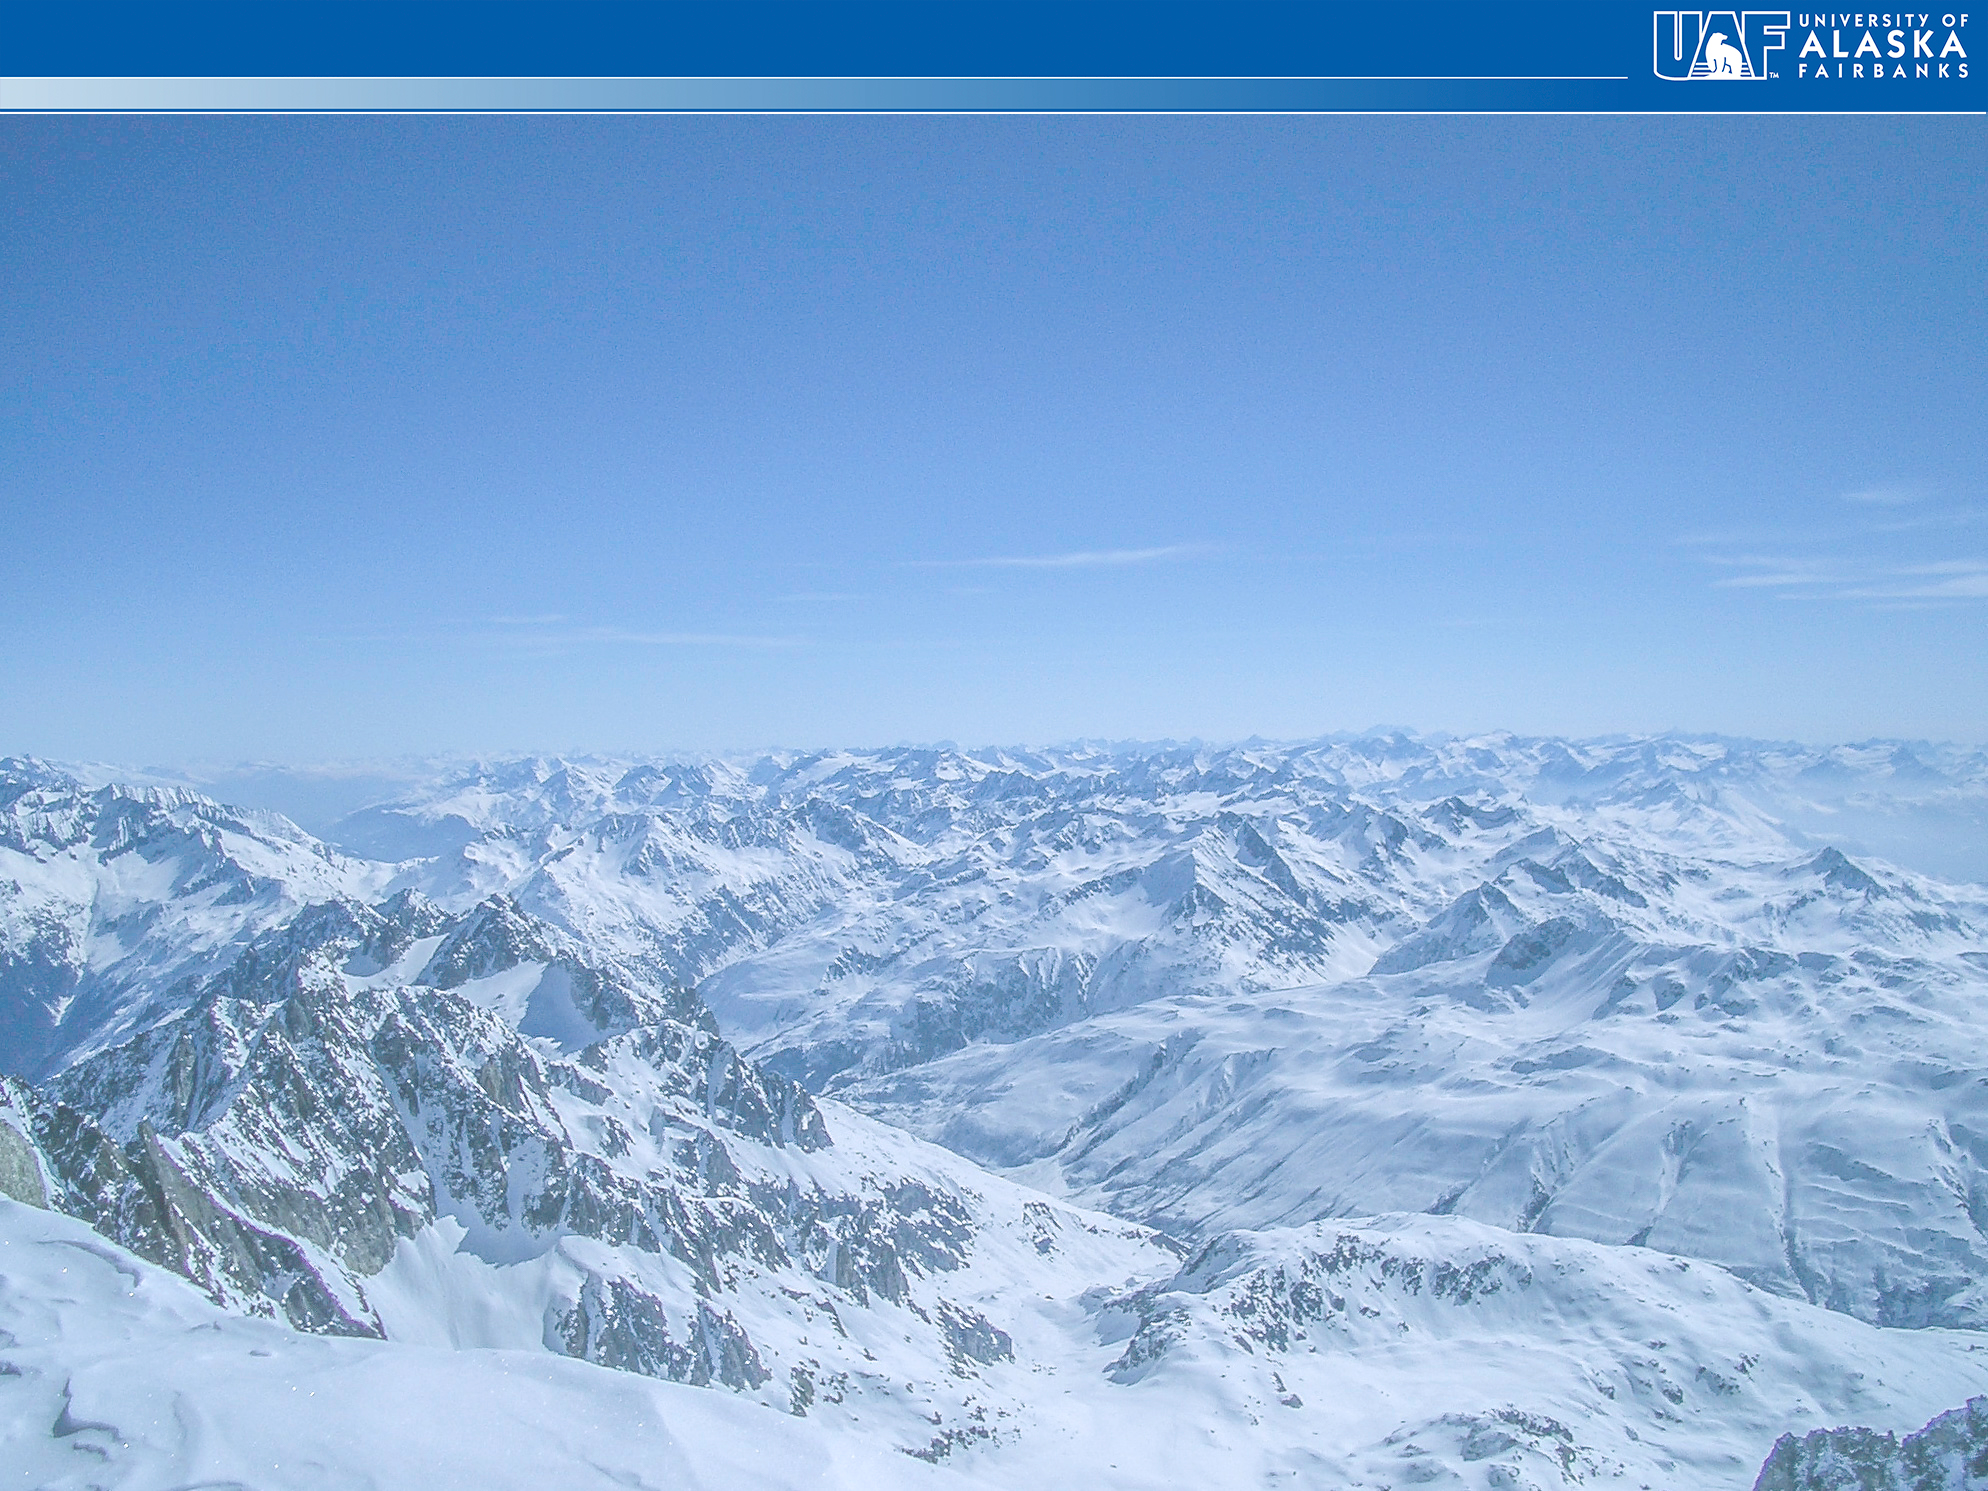
\includegraphics[width=\paperwidth]{galenstock_bg}};}
}

% insert titlepage
\begin{frame}
  \titlepage
  \note[item]{Who has ever seen a glacier?}
  \note[item]{Who has ever set foot on a glacier?}
  \note[item]{The picture here shows the view from on of my favorite places near}
  \note[item]{where I grew up}
\end{frame}

\setbeamertemplate{background canvas}
  {
} 


\setbeamertemplate{background canvas}
  {
     \tikz{\node[inner sep=0pt,opacity=1.] {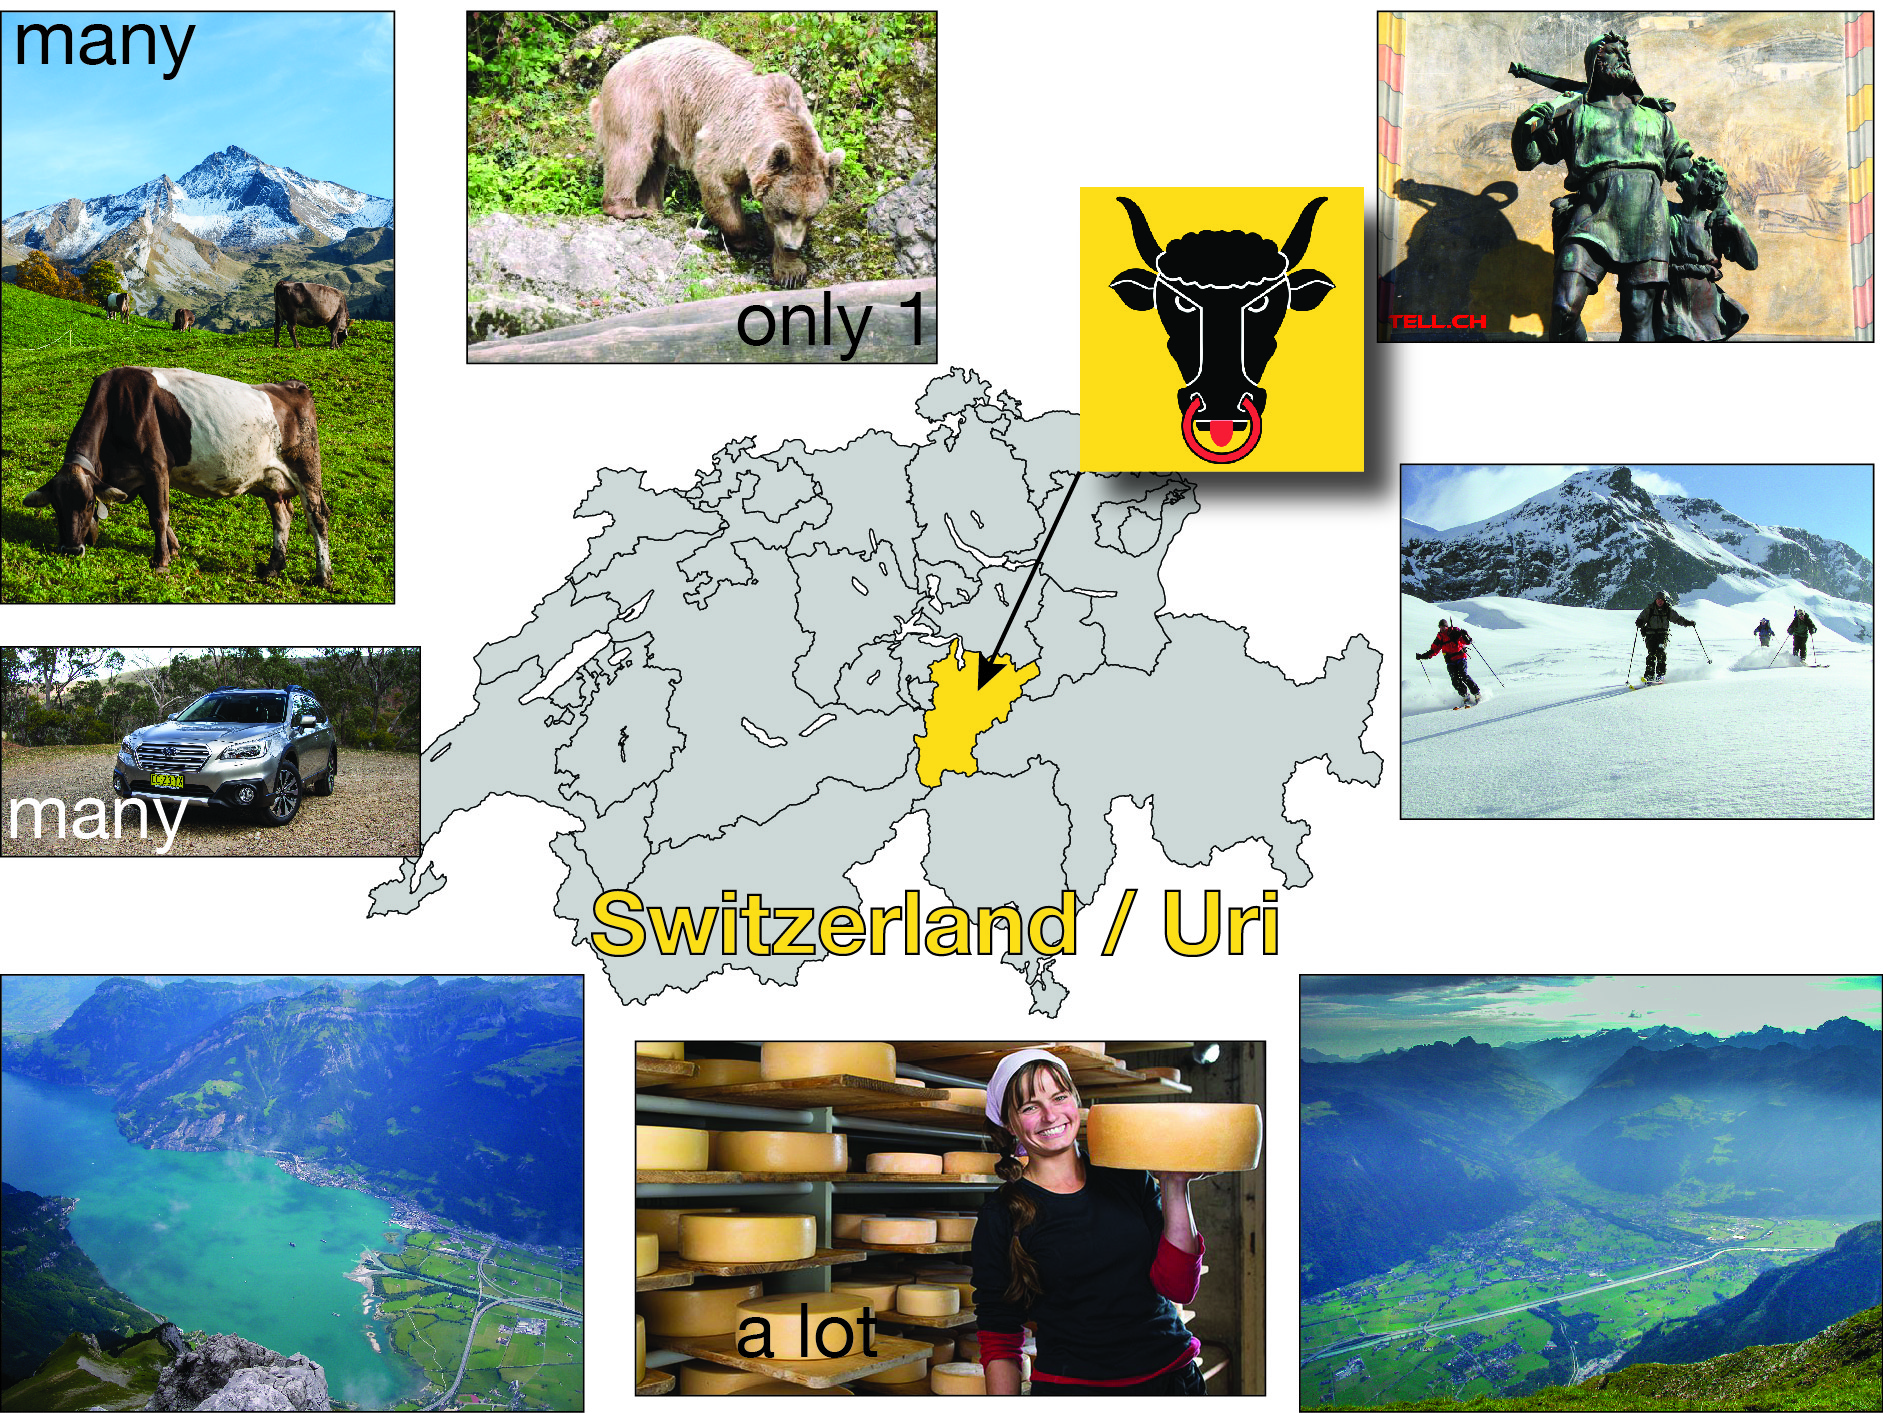
\includegraphics[width=\paperwidth]{uri-collage}};}
}

\begin{frame}[plain]
  \note[item]{I grew up in the heart of Switzerland, in the Kanton Uri---a Kanton is the equivalent to a State}
  \note[item]{Like Alaska, we have many Subarus}
  \note[item]{True to the stereotype, we have many cows in Uri and produce a lot of good cheese}
  \note[item]{We used to have bears}
  \note[item]{The last bear was shot in Uri in 1820 and you can still see the claws mounted to a house}
  \note[item]{Last year we had on bear roaming through Uri, which gave it some Alaska-feel}
  \note[item]{According to legend, William Tell was born in Uri, who freed us from the Austrian oppression in 1291}
  \note[item]{But first and foremost have a lot of mountains to climb and to ski}
\end{frame}

\setbeamertemplate{background canvas}
{
  \tikz{\node[inner sep=0pt,opacity=1.] {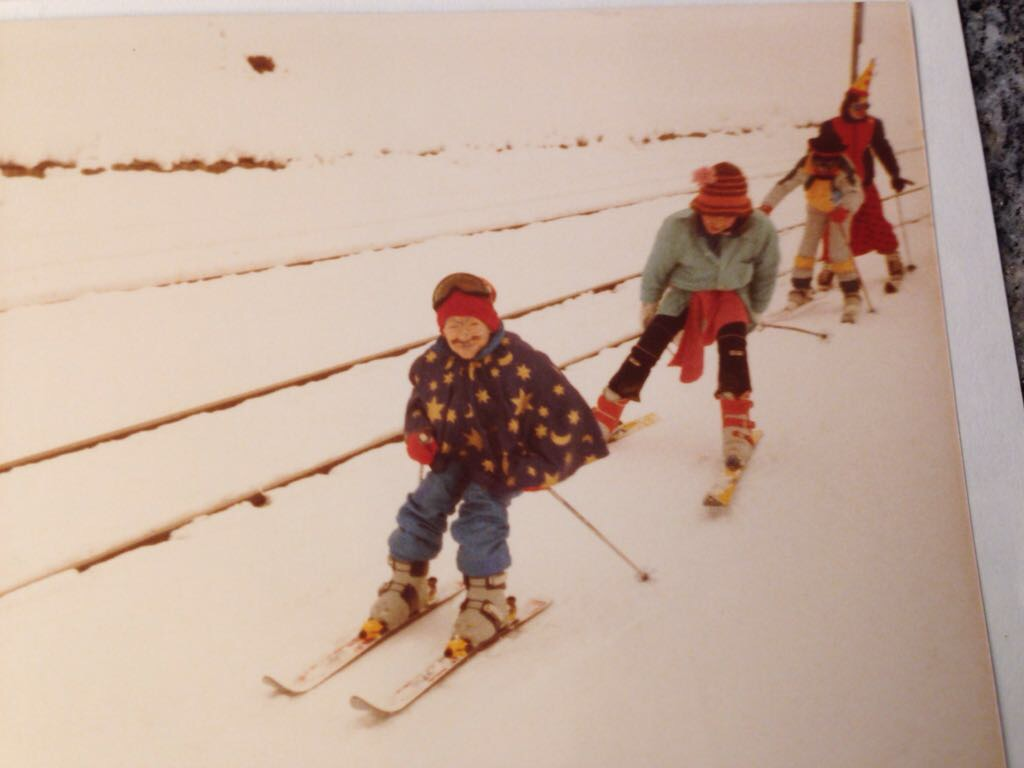
\includegraphics[width=\paperwidth]{andy-ski}};}
}

\begin{frame}[plain]
  \note[item]{So no surprise}
  \note[item]{I grew up on skis, I learned to downhill ski right after learning to walk}
  \note[item]{In Switzerland ``skiing'' always means downhill skiing, unlike here in Fairbanks where skiing usually means XC skiing}
\end{frame}



\setbeamertemplate{background canvas}
{
  \tikz{\node[inner sep=0pt,opacity=1.] {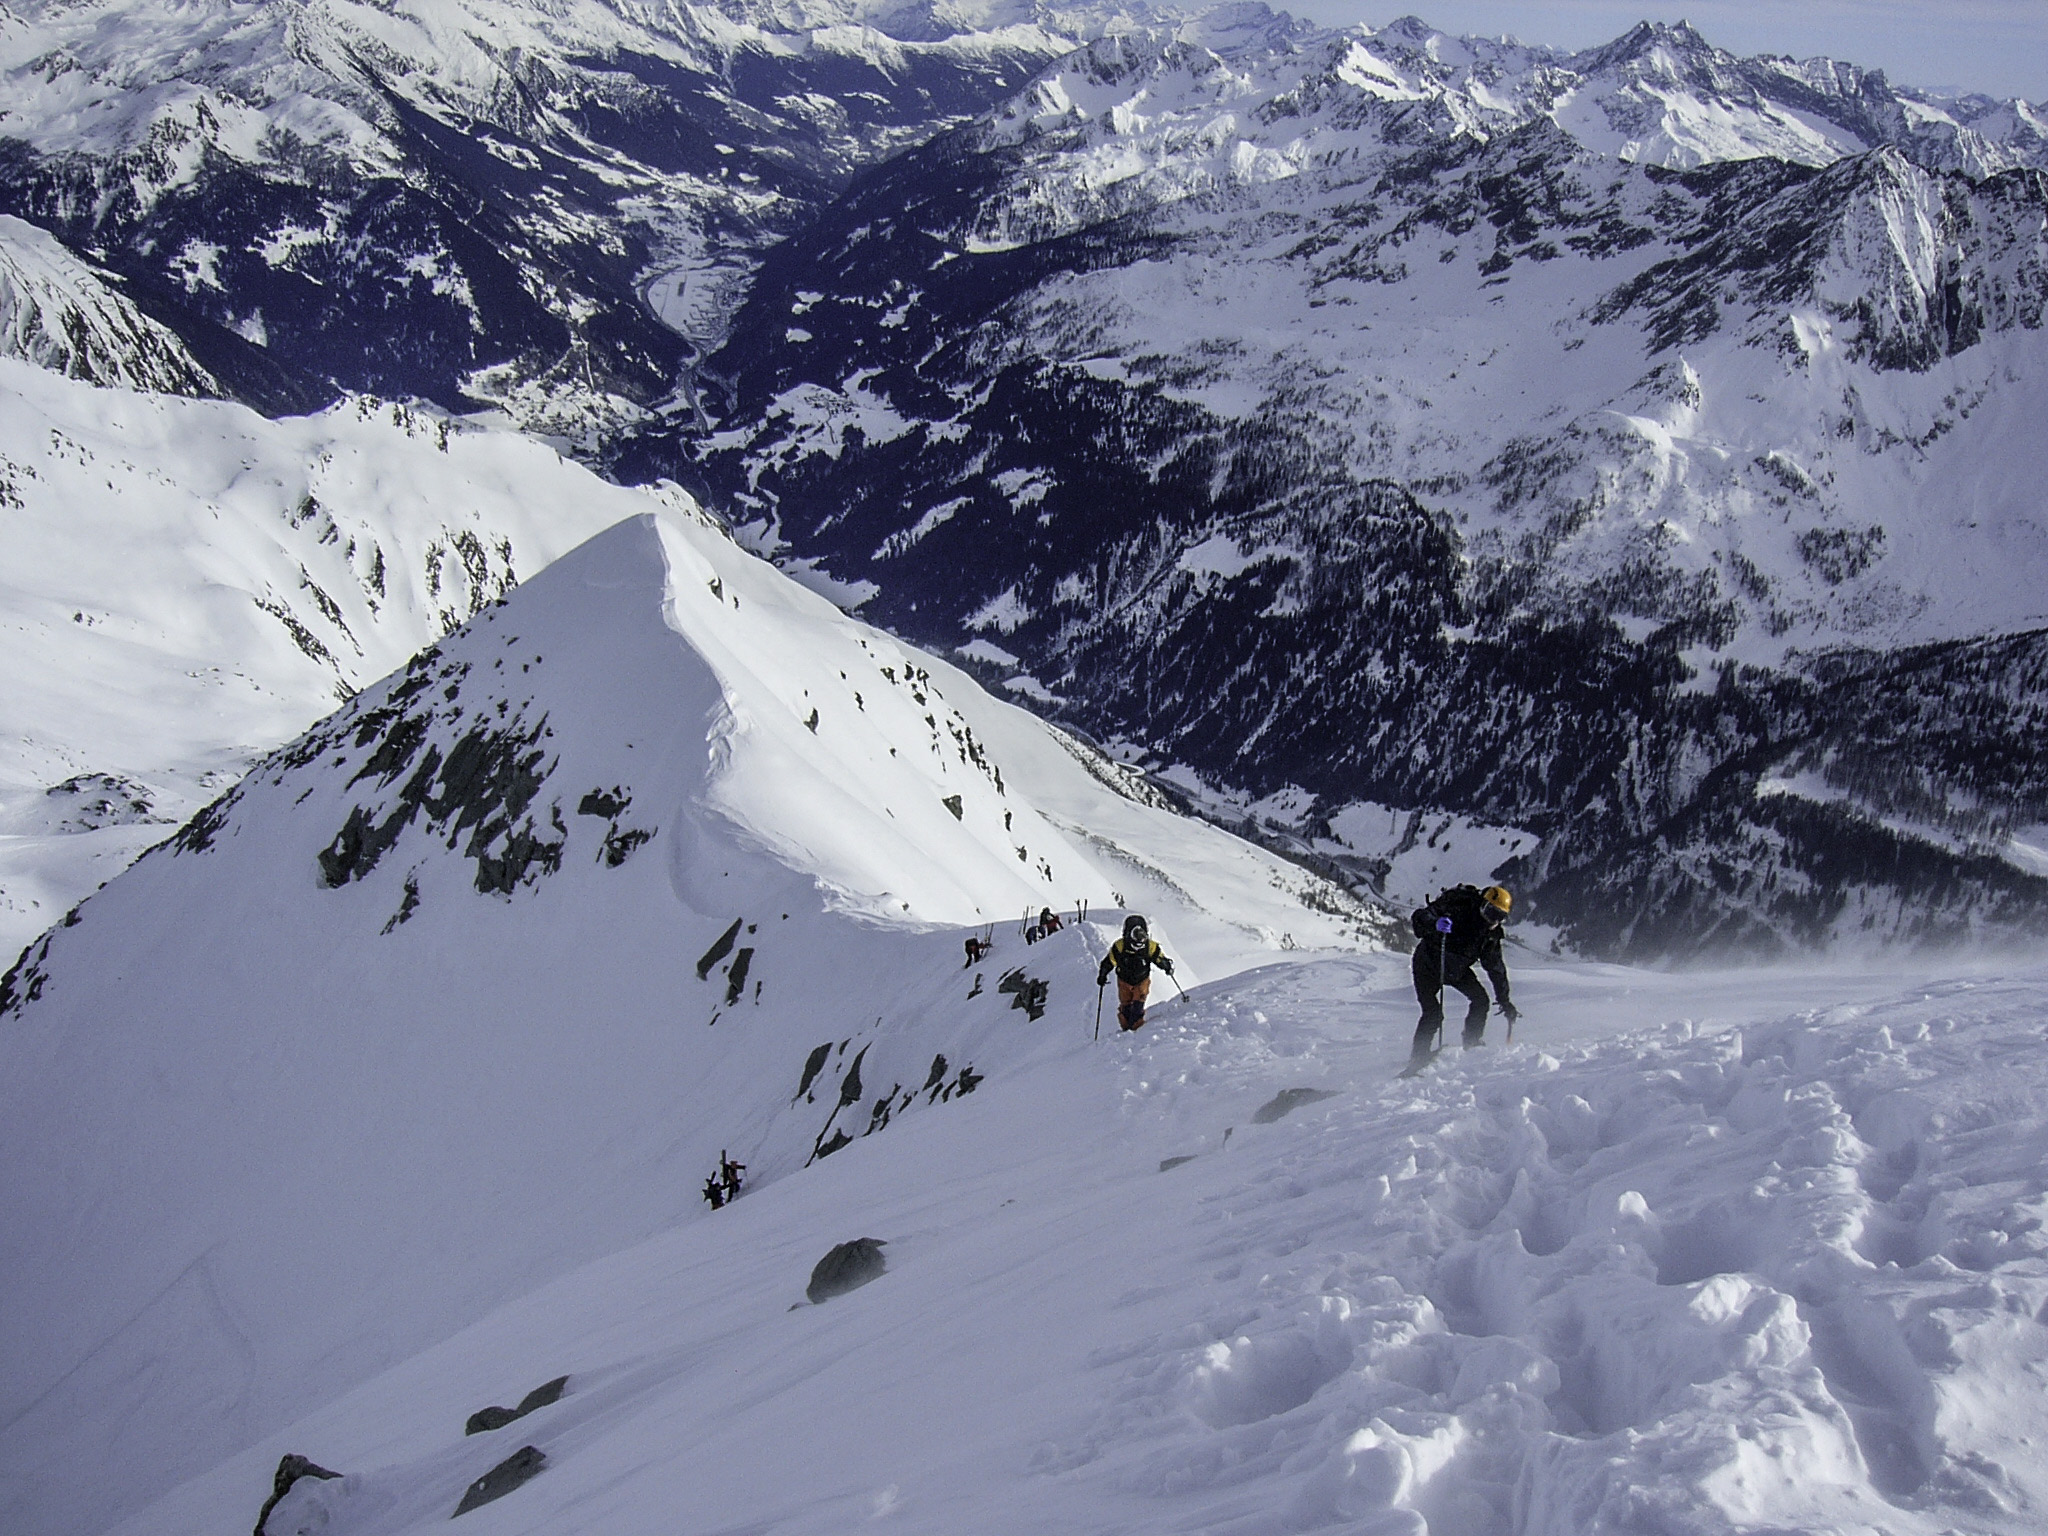
\includegraphics[width=\paperwidth]{ski-climb}};}
}

\begin{frame}[plain]
  \note[item]{When I was a bit older, I became tired of waiting for the next gondola}
  \note[item]{so started with ski mountaineering}
  \note[item]{and while spending my weekends in the mountains,}
  \note[item]{I started to notice change}
\end{frame}

\setbeamertemplate{background canvas}
{
  \tikz{\node[inner sep=0pt,opacity=1.] {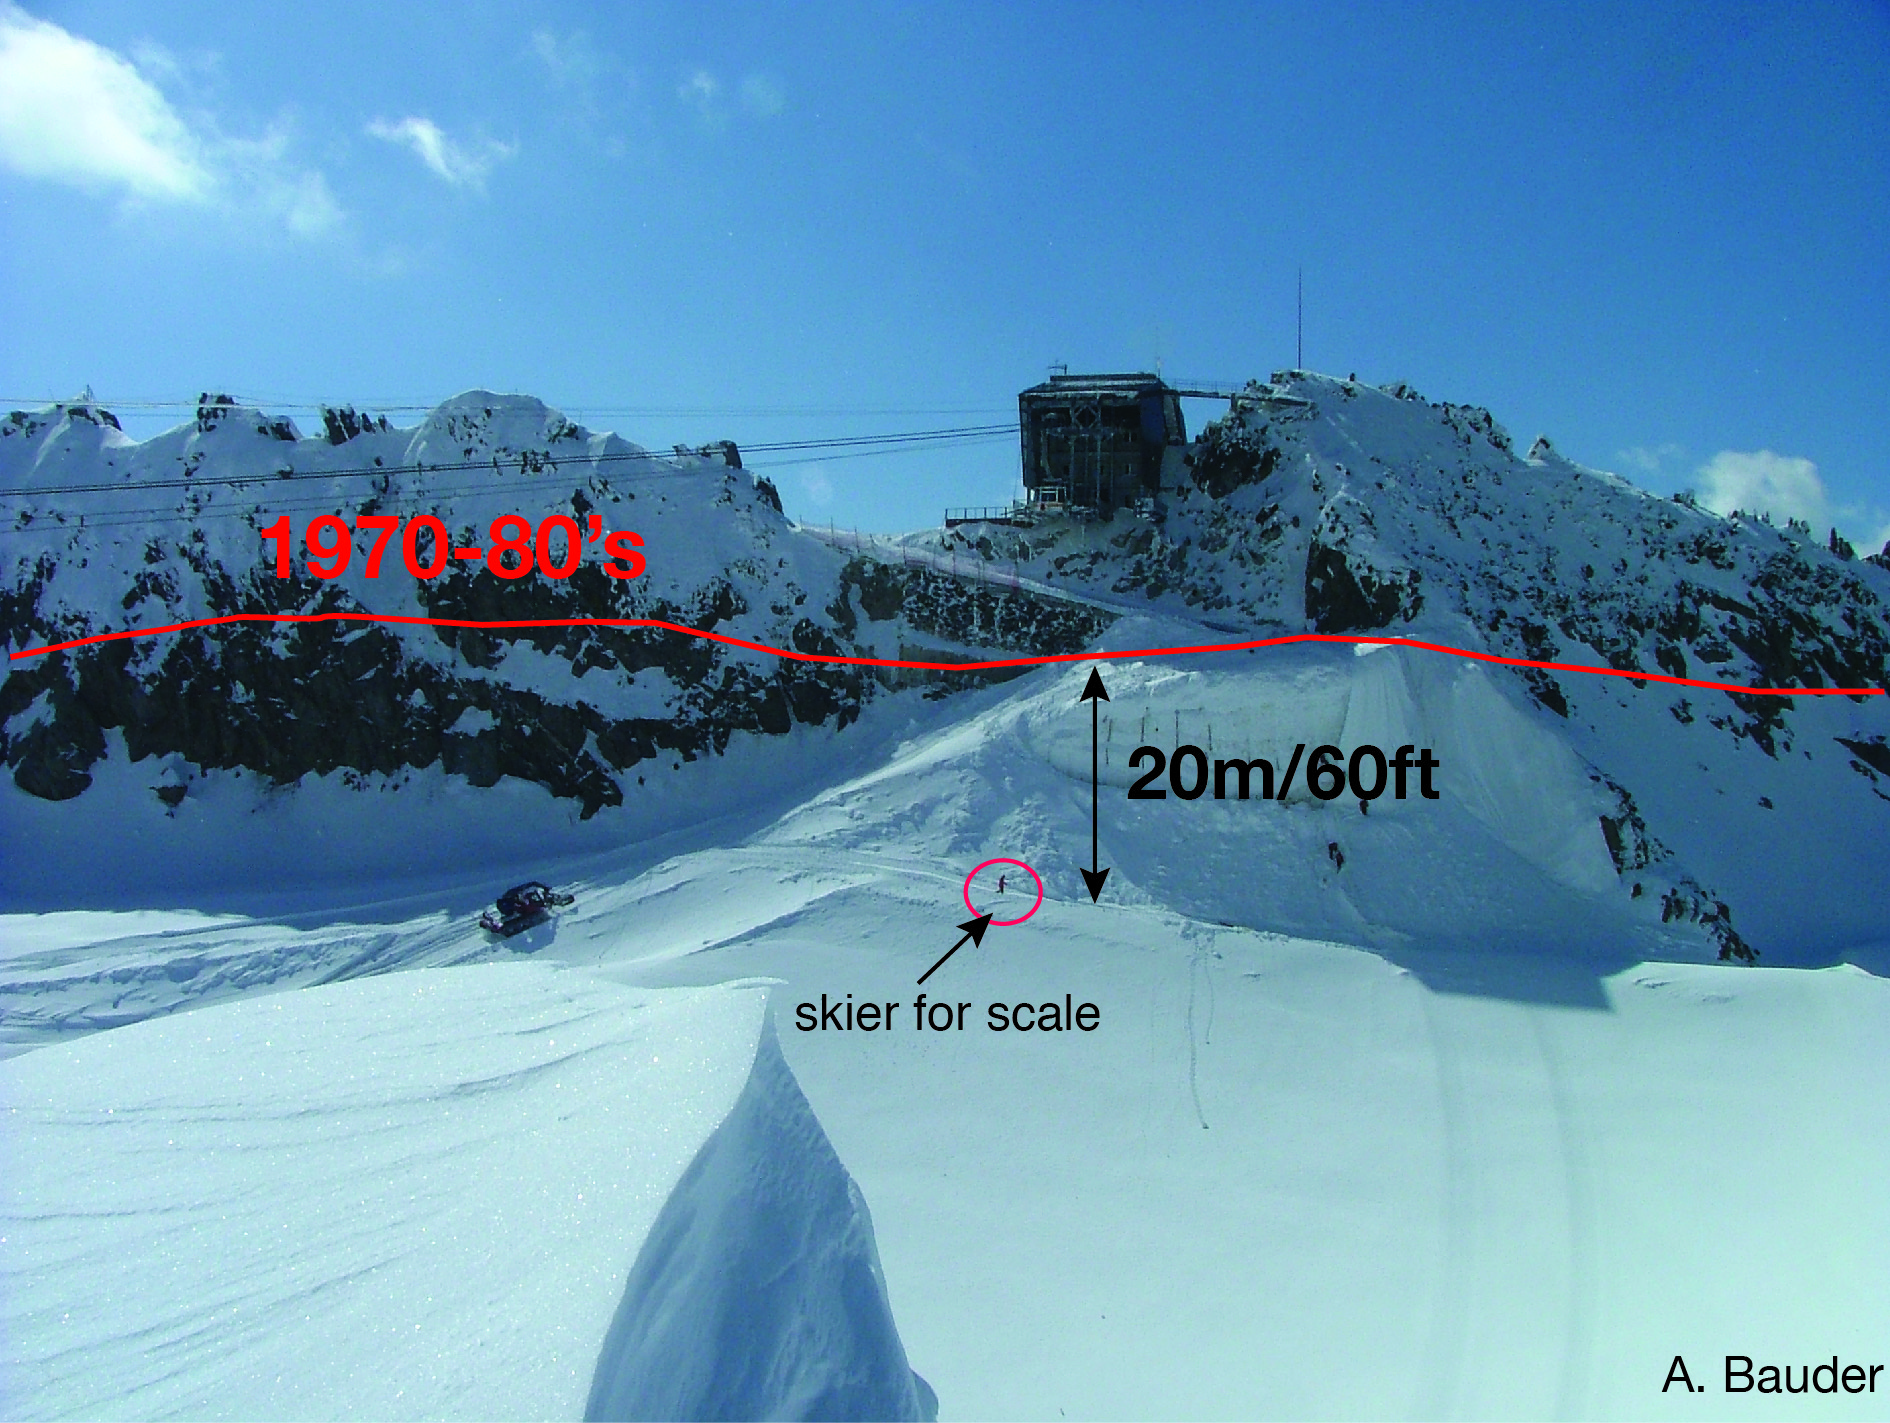
\includegraphics[width=\paperwidth]{gurschen-bauder}};}
}


\begin{frame}[plain]
  \note[item]{For example, when I was little we got out of the gondola}
  \note[item]{and we started to ski right on the glacier}
  \note[item]{However, in the past 2 or 3 decades, the glacier thinned by 20\,m or more}
  \note[item]{To get skiers on the glacier, they have to build a ramp out of snow every year}
  \note[item]{This is quite labor intensive and requires a lot of gas}
  \note[item]{Now, every spring ski patrol covers the ramp with a white tarp to preserve as much as possible}
  \note[item]{for the next winter}
  \note[item]{I asked myself: Are glaciers melting only where I grew up or is there more to it?}
  \note[item]{Is this happens somewhere else?}
  \note[item]{so, to answer this, I decided to study glaciology and climate science}
  \note[item]{but also it sounded like fun to study something that I can ski on\ldots}
  \note[item]{So during the rest of talk, I would like to give you my perspective of glaciers and glacier change}
  \note[item]{I will tell you about the health of Alaska's glaciers}
  \note[item]{and then show some of my current research}
\end{frame}
  

\setbeamertemplate{background canvas}
{
} 


\begin{frame}{Glaciers in Alaska}
  \begin{figure}
    \includegraphics<1>[width=0.8\textwidth]{gulkana1967}
    \includegraphics<2>[width=0.8\textwidth]{gulkana2016}
    \includegraphics<3>[width=0.8\textwidth]{gulkana2016-line}
    {\\ Fifty Years of Glacier Change in Alaska; USGS}
  \end{figure}
  \note[item]{Here's a photo I found on the USGS website on}
  \note[item]{50 years of glacier change in Alaska}
  \note[item]{Gulkana thinned and retreated}
\end{frame}


\setbeamertemplate{background canvas}
{
  \tikz{\node[inner sep=0pt,opacity=1]{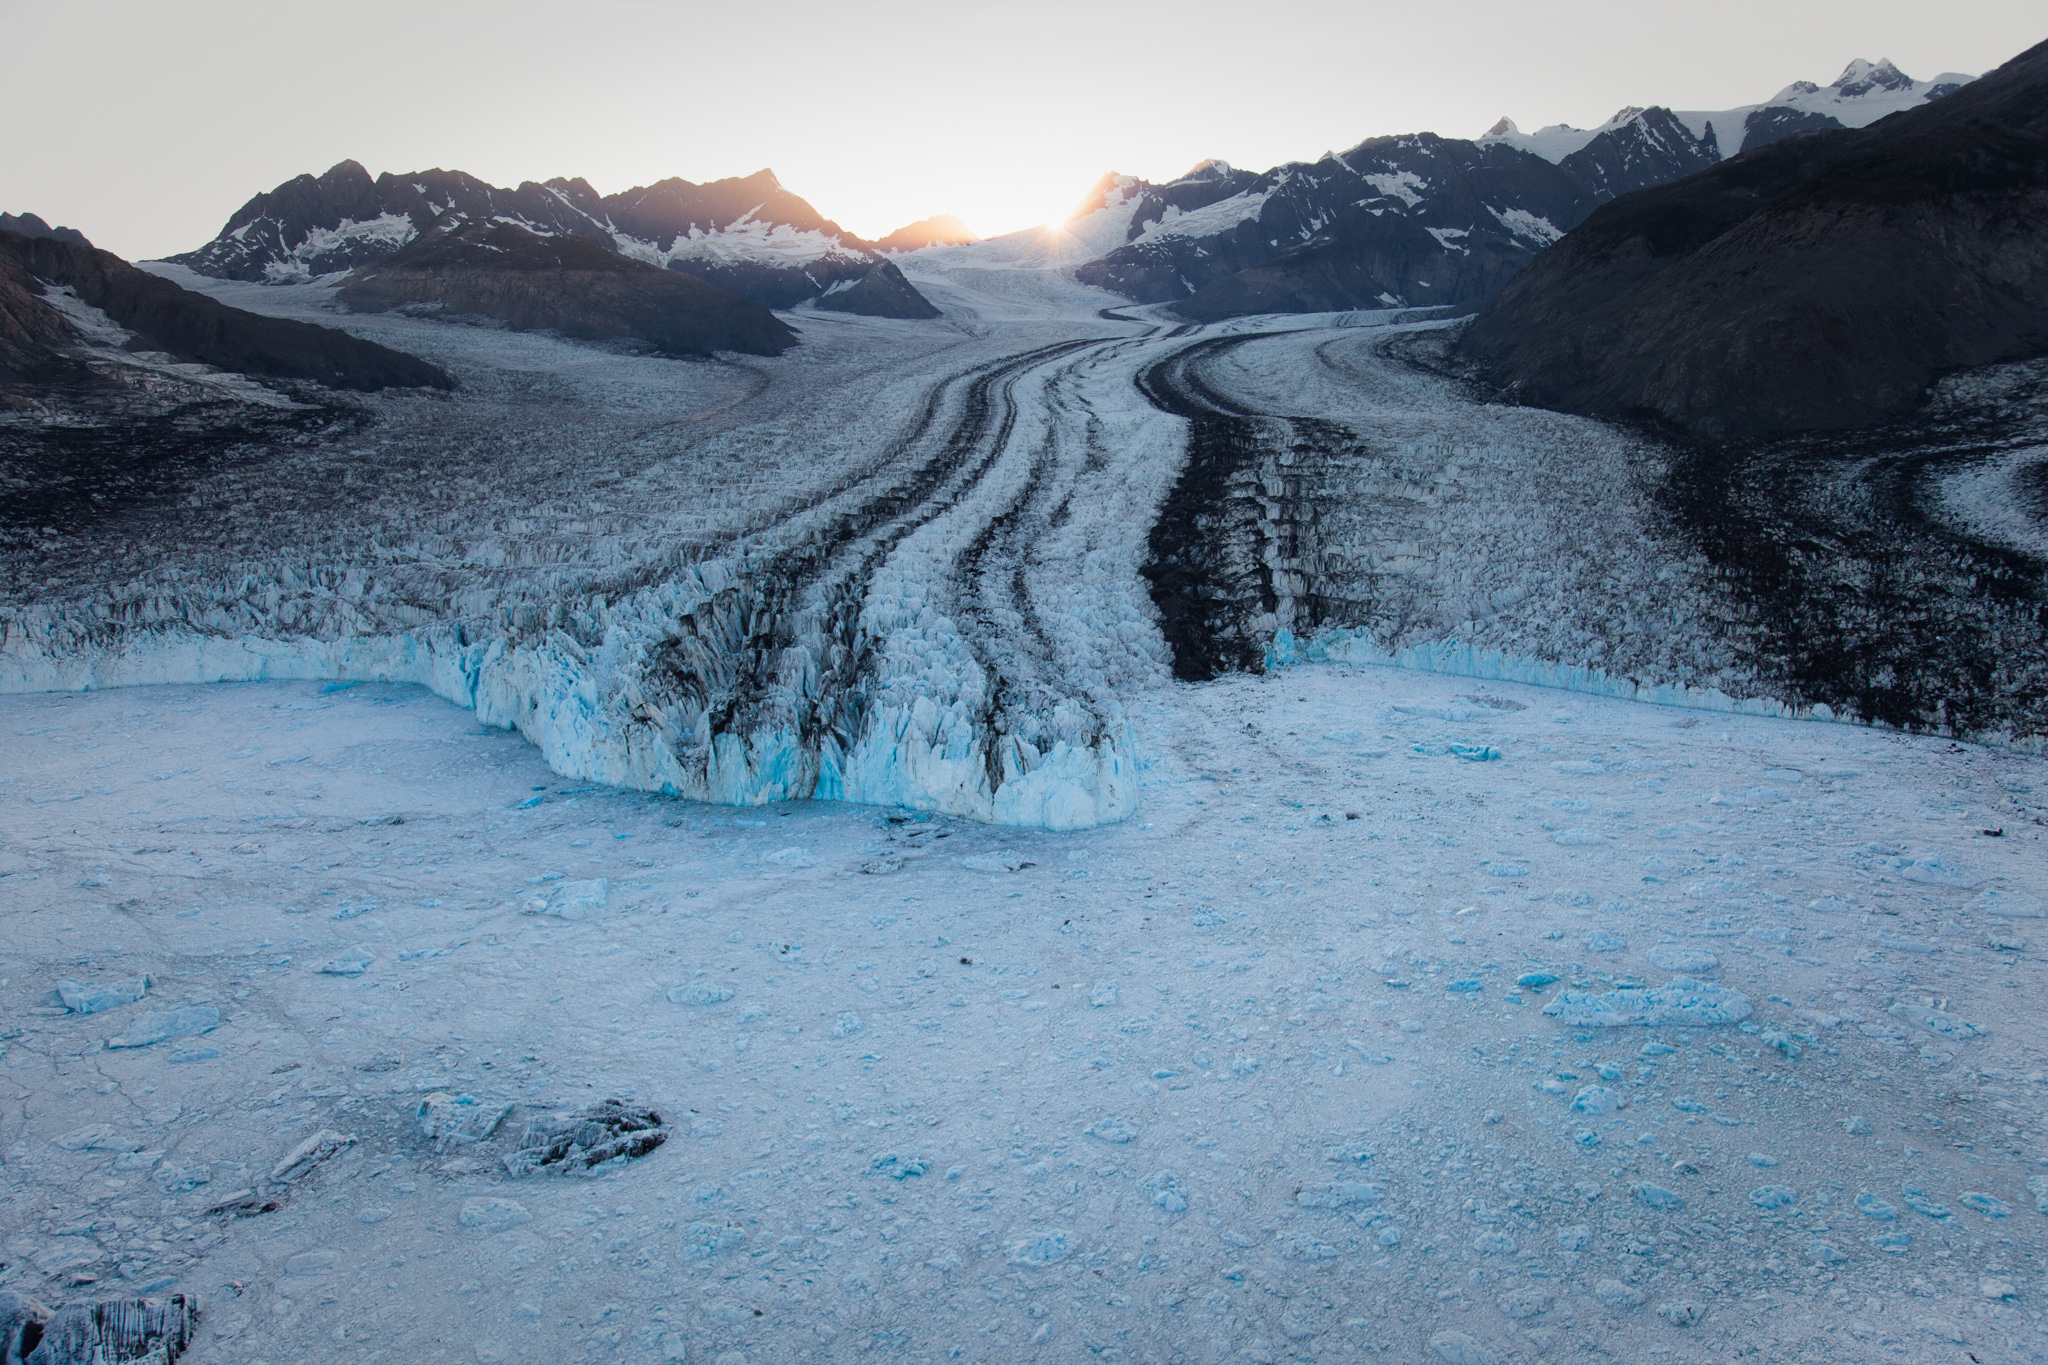
\includegraphics[width=\paperwidth,height=\paperheight]{columbia-glacier-2010}};}
}

\begin{frame}{Columbia Glacier}
  \note[item]{Who has been to Columbia Glacier near Valdez?}
  \note[item]{This photo is from an Alaska Tourism website and it dates to 2010.}
  \note[item]{You can see Columbia Glacier flowing into the ocean}
  \note[item]{The vertical cliff here is called the glacier terminus or the calving front}
\end{frame}

\setbeamertemplate{background canvas}
{
}



\begin{frame}{Melting Glaciers in Alaska: Columbia Glacier}
  \includemedia[
  width=12cm,
  activate=pageopen,
  addresource=columbia-eis.mov,
  flashvars={source=columbia-eis.mov
    &modestbranding=1 % no YT logo in control bar
    &autohide=0
    &showinfo=0
    &rel=0
    % controlbar autohide
    % no title and other info before start
    % no related videos after end
  }
]{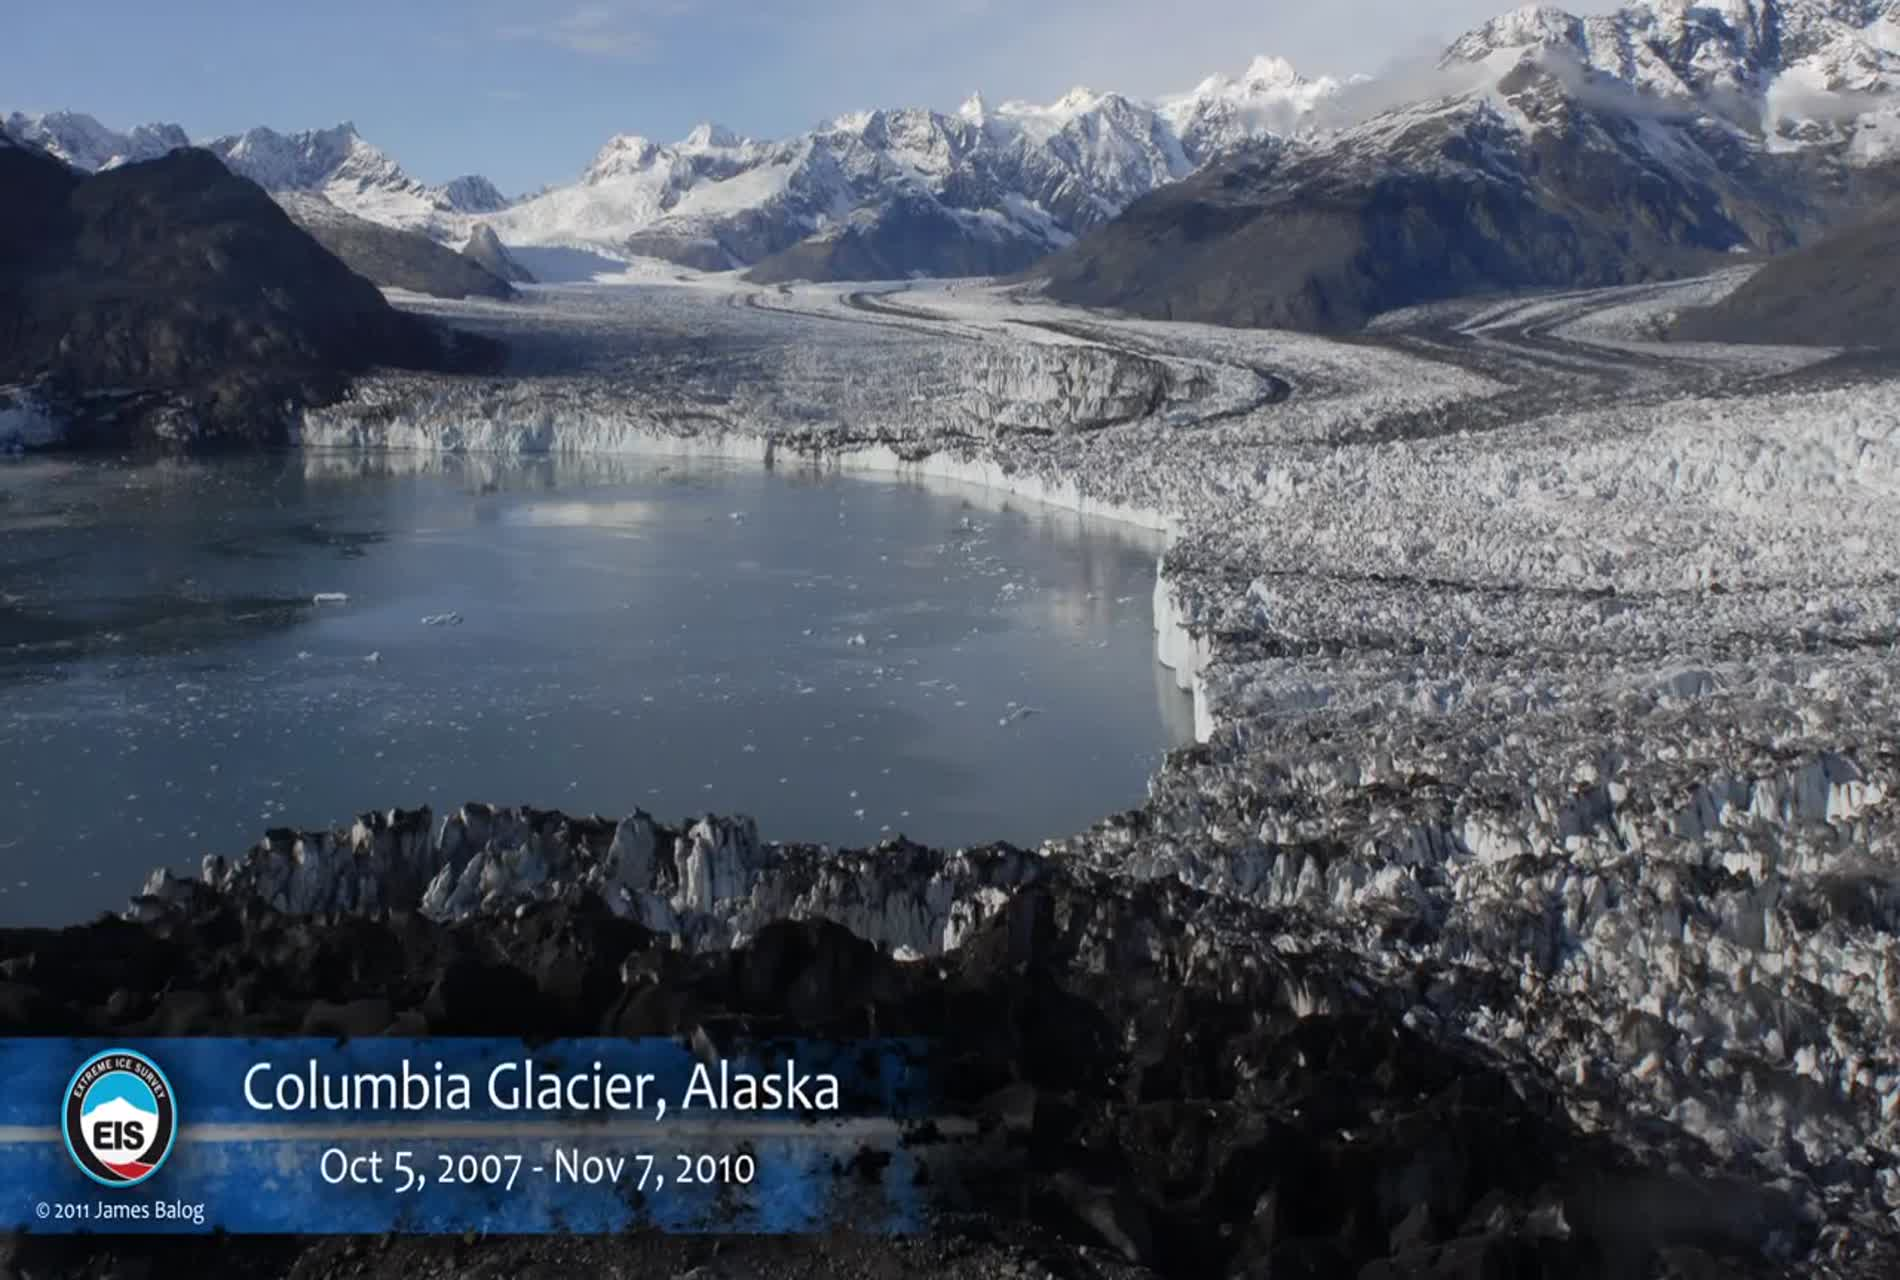
\includegraphics[width=12cm]{columbia-eis}}{VPlayer.swf}
  \note[item]{Here is a video put together from time lapse photography by James Balog from EIS.}
  \note[item]{Columbia Glacier looks like a river of frozen ice, all cracked up, flowing into the ocean}
  \note[item]{When Columbia Glacier was first surveyed by British explorers in 1794}
  \note[item]{it extented to Heather Bay and held that position until 1980.}
  \note[item]{In 1980s, Columbia Glacier started a rapid that continues today.}
  \note[item]{Since 1986, Colmbia Glacier retreated by more than 20 kilometers.}
  \note[item]{It shows how fast the glacier retreated between 2007 and 2010.}
  \note[item]{In fact, Columbia Glacier retreated so fast}
  \note[item]{that they had to reposition the camera three times}
\end{frame}


\setbeamertemplate{background canvas}
{
  \tikz{\node[inner sep=0pt,opacity=0.75] {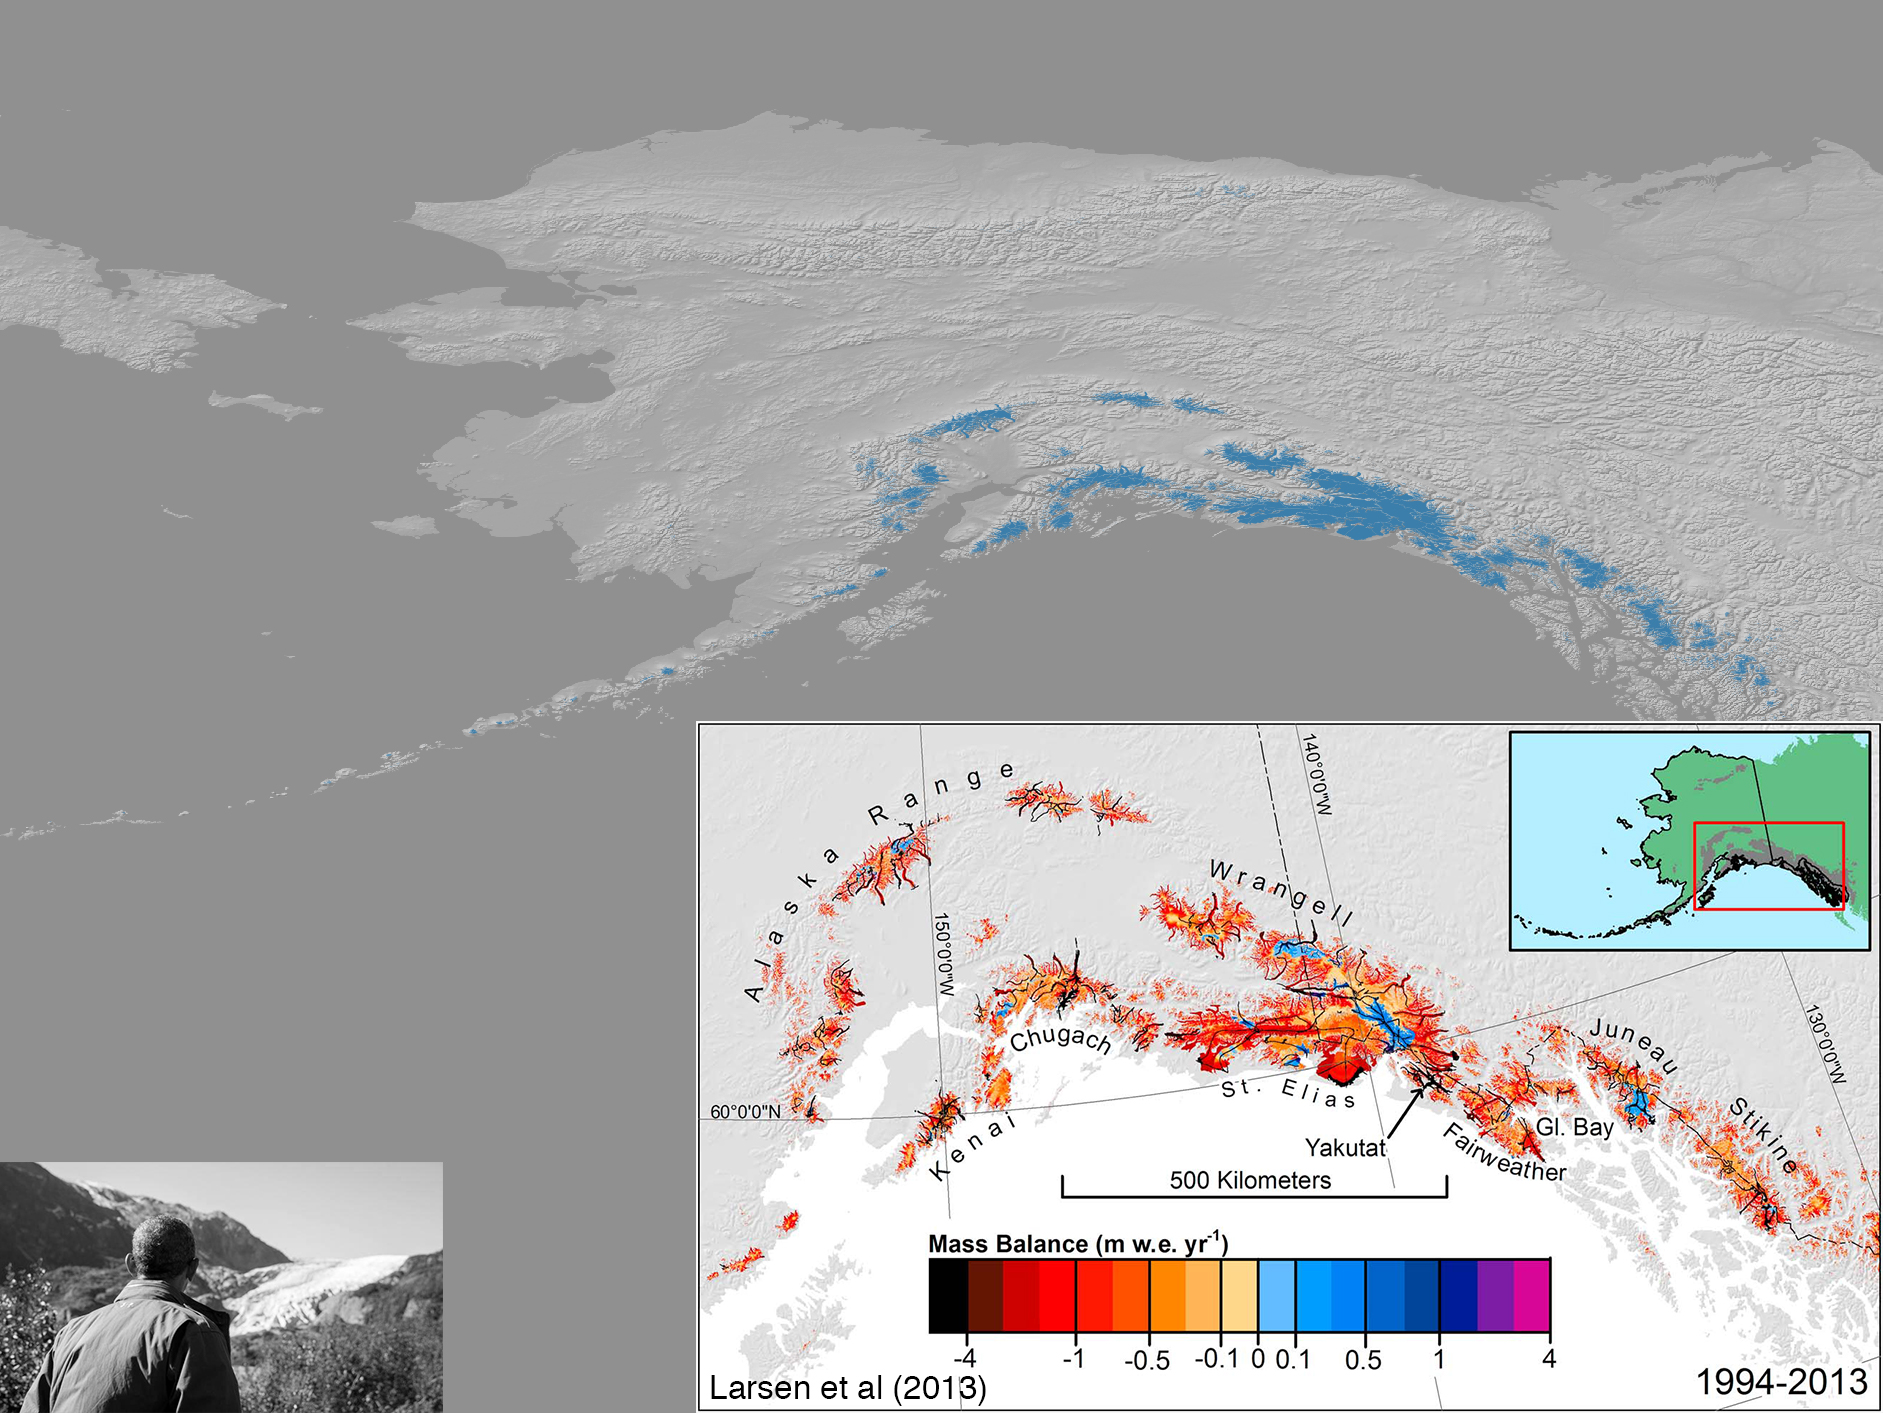
\includegraphics[width=\paperwidth]{ak_glacierized_area_melt_16x12}};}
}

\begin{frame}{Melting Glaciers in Alaska}
  \begin{itemize}
  \item total mass loss 1994--2013 from AK glaciers: 75$\pm$11 Gt/yr loss $\Rightarrow$ 5\,cm (2\,in) layer of water covering Alaska
  \end{itemize}
  \note[item]{Explain thinning and mass loss}
  \note[item]{Columbia Glacier is not alone}
  \note[item]{As recent study by UAF's Chris Larsen and others shows that many glaciers are melting}
  \note[item]{The red colors indicate glaciers that have lost mass between 1994 and 2013}
  \note[item]{while blue color indicate mass gain}
  \note[item]{there are many more glaciers losing mass than gaining mass}
  \note[item]{Between 94 and 2013, Alaskan glaciers lost a combined 75 Gt per year}
  \note[item]{How much are 75 giga ton?}
  \note[item]{If you spread 75 Gt of water evenly over Alaska}
  \note[item]{and here we assume Alaska is flat}
  \note[item]{we would stand in 5cm deep water}
  \note[item]{or, if we combine all 20 years, would be standing in about a meter of water}

\end{frame}

\setbeamertemplate{background canvas}
{
}



\begin{frame}{Melting Glaciers Everywhere: The Biggest Losers}
  \begin{figure}
    {Alaska \qquad---\qquad West Greenland \qquad---\qquad West Antartica}
    \\[1em]
    \includegraphics<1>[width=1\textwidth]{world-grace-2002-2016}
  \end{figure}
  \note[item]{But maybe Switzerland and Alaska are the exception?}
  \note[item]{Glaciers are melting worldwide}
  \note[item]{This figure shows glacier mass loss world wide}
  \note[item]{Again, red colors indicate mass loss}
  \note[item]{High mountain Asia hard to resolve}
  \note[item]{The biggest red areas are Alaska, Greenland, and West Antartica}
  \note[item]{These are the biggest losers right now}
\end{frame}

\setbeamertemplate{background canvas}
{
  \tikz{\node[inner sep=0pt,opacity=.6] {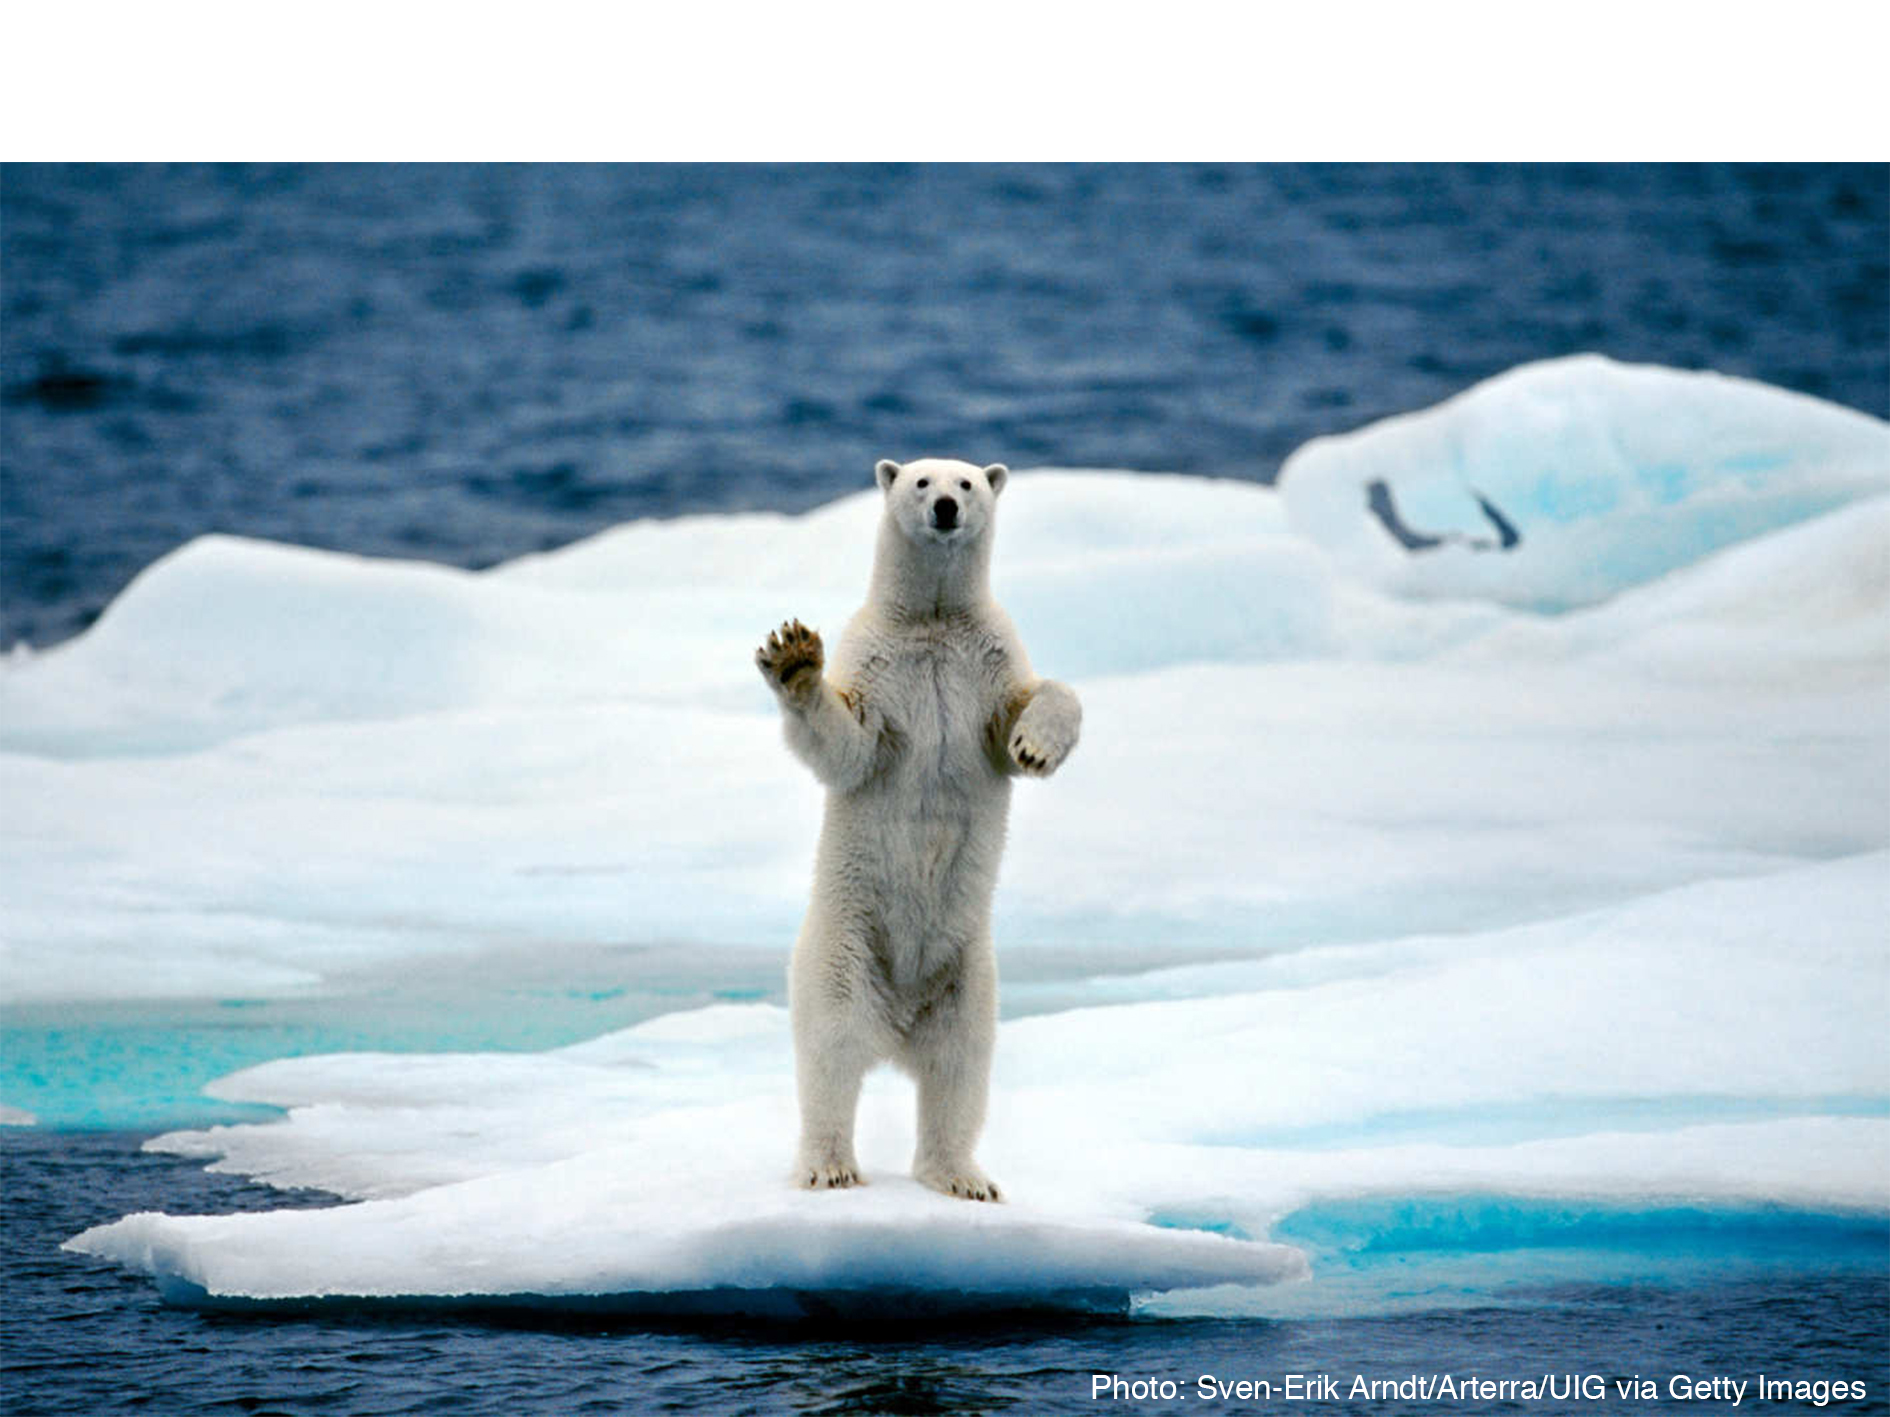
\includegraphics[height=\paperheight,width=\paperwidth]{polar-bear-wcredit}};}
}


\begin{frame}{}
  \centering{\alert{\textbf{``Hasn't the Climate Changed Before?''}}}
  \note[item]{But wait}
  \note[item]{aren't glaciers and the climate constantly changing}
  \note[item]{What's so special about today?}
  \note[item]{That's probably the number one question}
  \note[item]{I get from a seat neighbor in airplane}
  \note[item]{So let me try to walk you through the climate of the past}
  \note[item]{and how the climate influences glaciers}
\end{frame}

\setbeamertemplate{background canvas}
{
}


\begin{frame}{Glacials and Interglacials}
      \begin{figure}
        \includegraphics<1>[height=8.2cm]{ice-age-movies}
      \end{figure}
  \note[item]{As we learned from Hollywood}
  \note[item]{there have been Ice Ages and Meltdowns}
  \note[item]{or as we call it: glacials and interglacials}
\end{frame}

\setbeamertemplate{background canvas}
{
  \tikz{\node[inner sep=0pt,opacity=1] {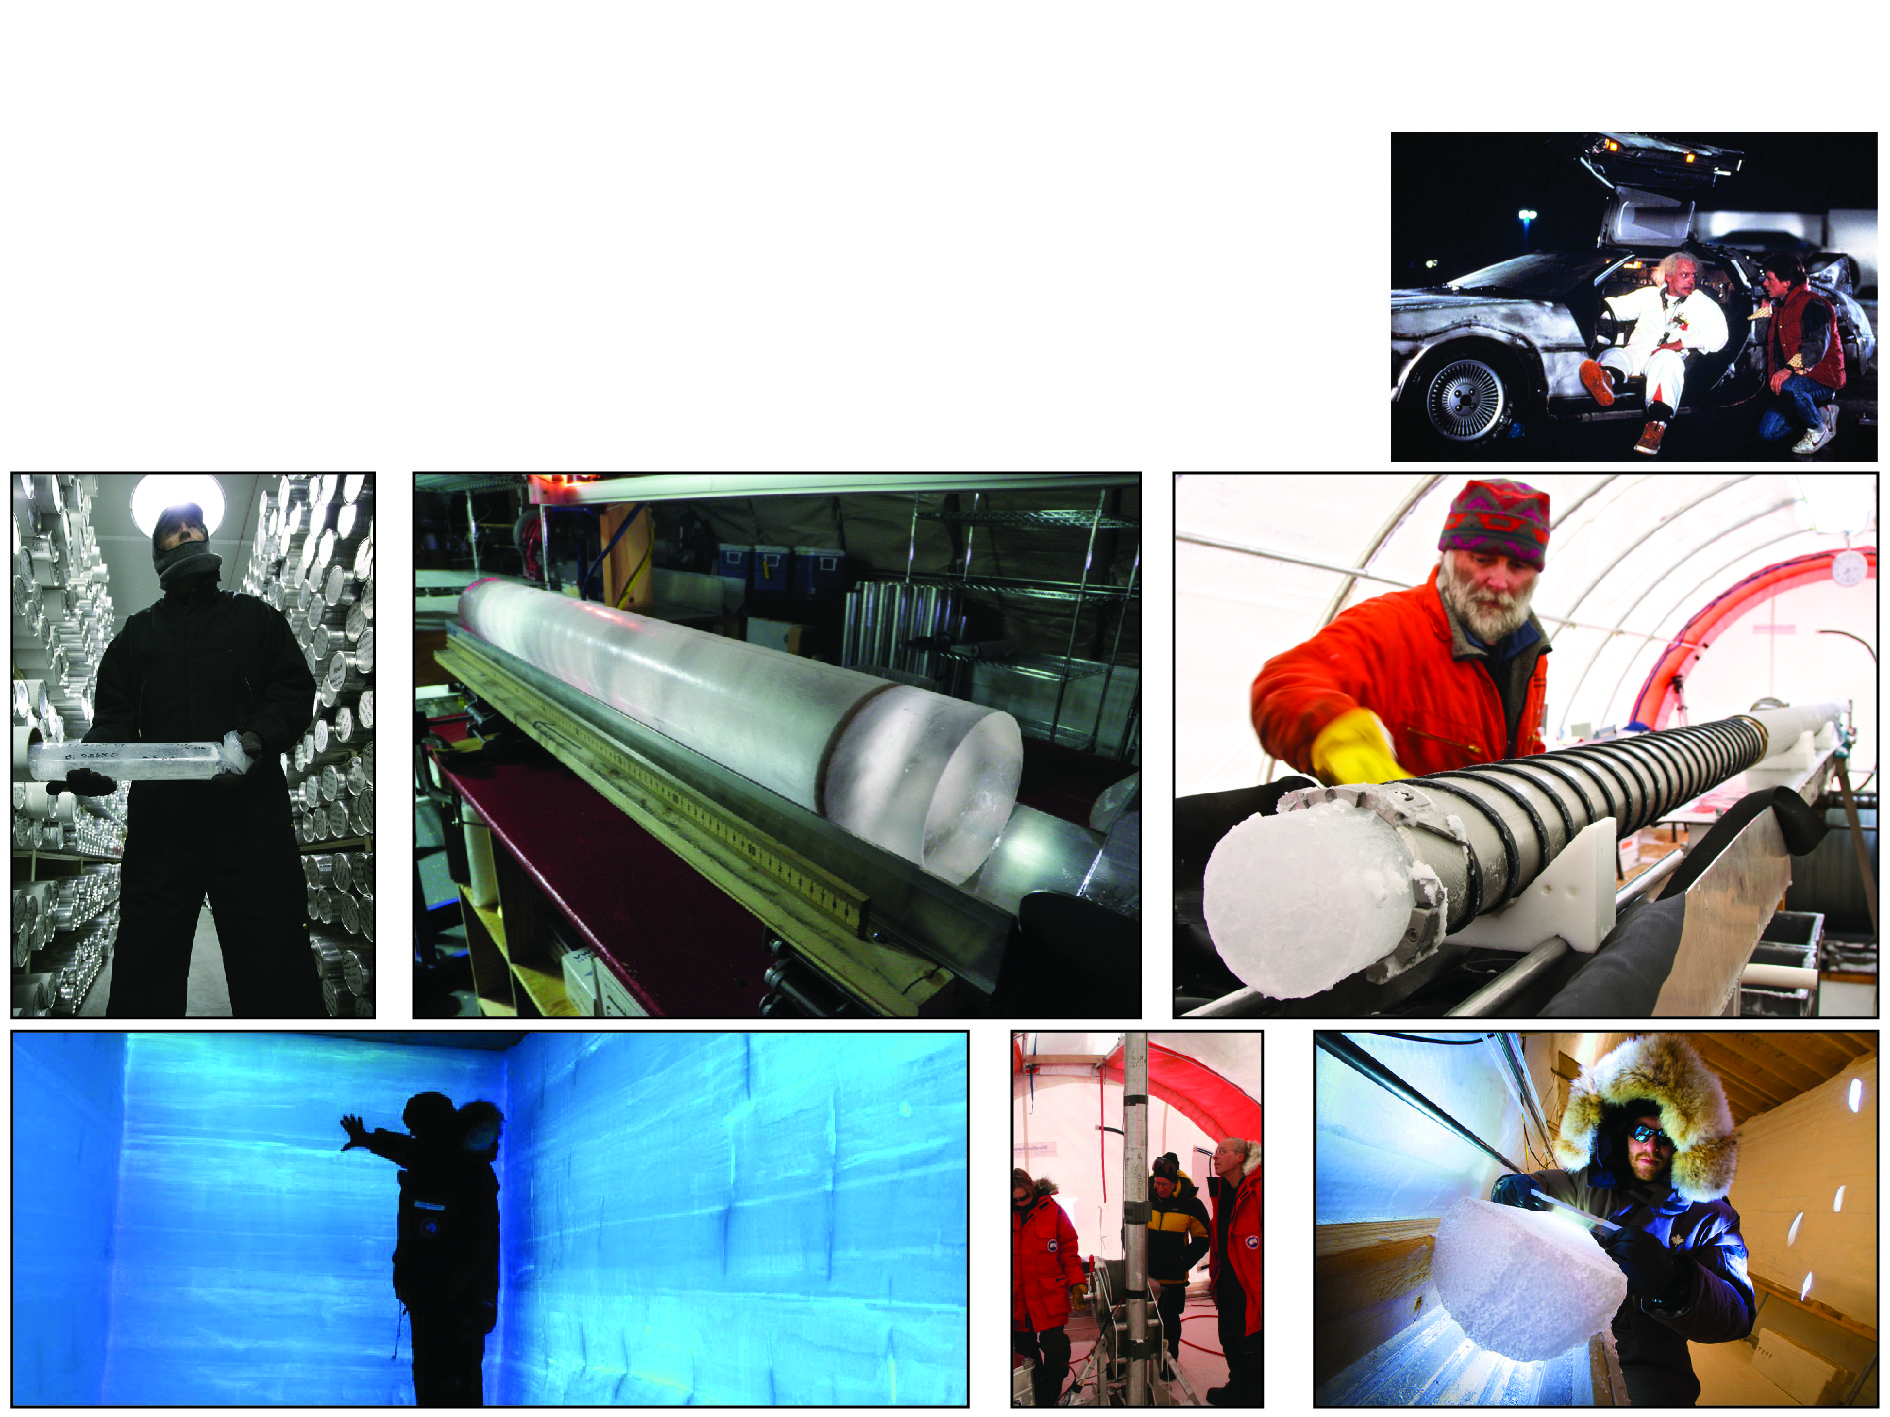
\includegraphics[height=\paperheight,width=\paperwidth]{ice-core-collage}};}
}

\begin{frame}{Ice Cores: The 2-mile Time Machine}
  \note[item]{We know about glacials and interglacials from}
  \note[item]{geologic evidence and from ice cores}
  \note[item]{What is an ice core and what can it do for you?}
  \note[item]{In cold areas such as Greenland and Antarctica}
  \note[item]{snow falls every year on top of the snow from the previous year}
  \note[item]{building layer after layer, as you can see in the photo here}
  \note[item]{when the weight of the overlying snow is heavy enough, the snow turns into ice}
  \note[item]{during the process, tiny bubbles of air are being trapped within the ice}
  \note[item]{the air in those bubbles contains a lot of information}
  \note[item]{about the climate of the year when the snow fell}
  \note[item]{An ice core is like a big archive that}
  \note[item]{stores information about past climate}
  \note[item]{each bubble is a time capsule}
  \note[item]{Ice cores from Greenland and Antartica are up to 2 mile deep}
  \note[item]{the deeper you go, the older the ice gets}
  \note[item]{climate scientists have analyzed ice that is up to 800,000 years old}
  \note[item]{This gives us a pretty good picture about climate varibility over almost a million years}
\end{frame}

\setbeamertemplate{background canvas}
{
  \tikz{\node[inner sep=0pt,opacity=0.4] {
\includegraphics[height=\paperheight,width=\paperwidth]{ice-age}};}
}

\begin{frame}{Climate History}
  \vspace{.15cm}
  \begin{figure}
    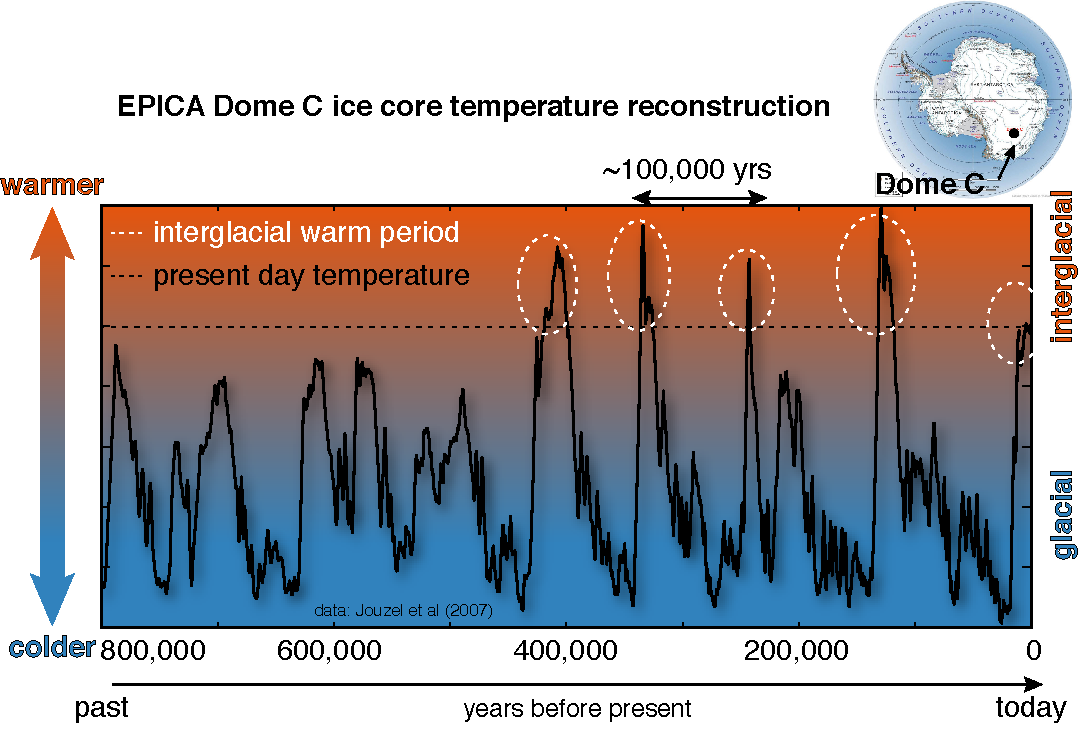
\includegraphics[width=\textwidth]{epica-temp}
  \end{figure}
  \note[item]{Let's look at temperature changes}
  \note[item]{What is this, explain time axis}
  \note[item]{We see that most of the time, it was cold and we were in an Ice Age}
  \note[item]{But find 5 distinct warm periods during the past half a million years, about 100,000 years apart}
  \note[item]{and we are currently in the fifth warm period or interglacial that started about 12,000yrs ago}
  \note[item]{There have been times when it was warmer than today}
  \note[item]{but the last time it was warmer was more the 100,000yrs ago }
  \note[item]{This cycle of glacials and interglacials is driven by how much sun light the Northern Hemisphere receives}
  \note[item]{These are the Milankovitch cycle}
  \note[item]{The physics behind this is well understood but would take up a whole other talk}
\end{frame}


\setbeamertemplate{background canvas}
{
}

\begin{frame}{What makes the past 100\,yrs so special?}
  \begin{figure}
    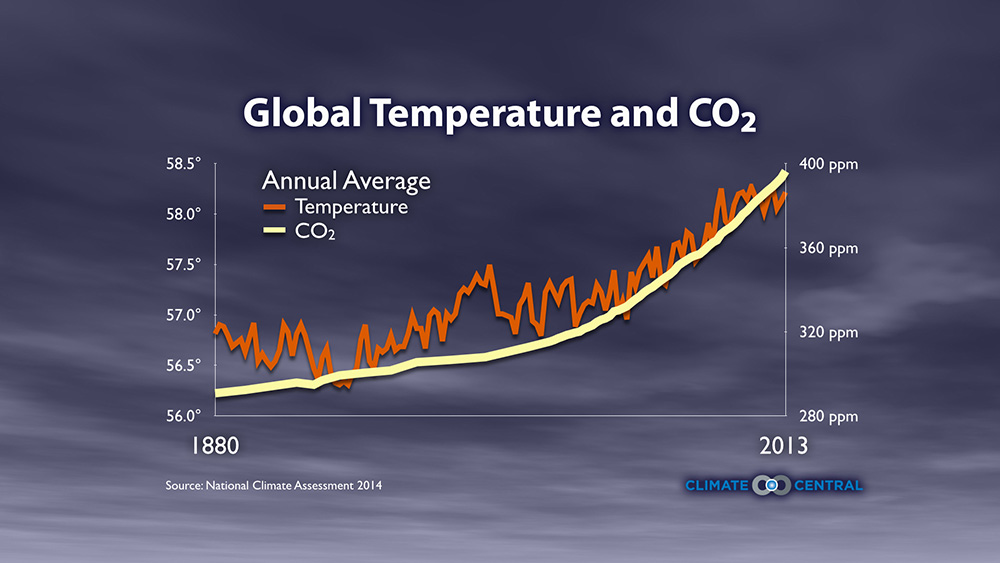
\includegraphics[width=\textwidth]{Global_Temp_and_CO2}
  \end{figure}
  \note[item]{Since I explained in the previous slide that whether we are in}
  \note[item]{an Ice Age or a warm period depends on how much sun we are receiving}
  \note[item]{one could suggest that increased solar activity is driving the current glacier mass loss}
  \note[item]{But if we look at sun activity, the sun activity has not increased considerably}
  \note[item]{so the sun is not the culprit, what else could it be?}
  \note[item]{Around the times of the Civil War, scientists discovered the Greenhouse effect}
  \note[item]{and by the end of the 19th century, we already knew that adding carbon dioxide to the atmosphere}
  \note[item]{will warm our planet}
  \note[item]{This relationship is illustrated in this figure here.}
  \note[item]{The orange curve shows temperature and the yellow curve shows CO2}
  \note[item]{And you can see that temperature follows CO2 quite well}
\end{frame}

  

\setbeamertemplate{background canvas}
  {
     \tikz{\node[inner sep=0pt,opacity=1] {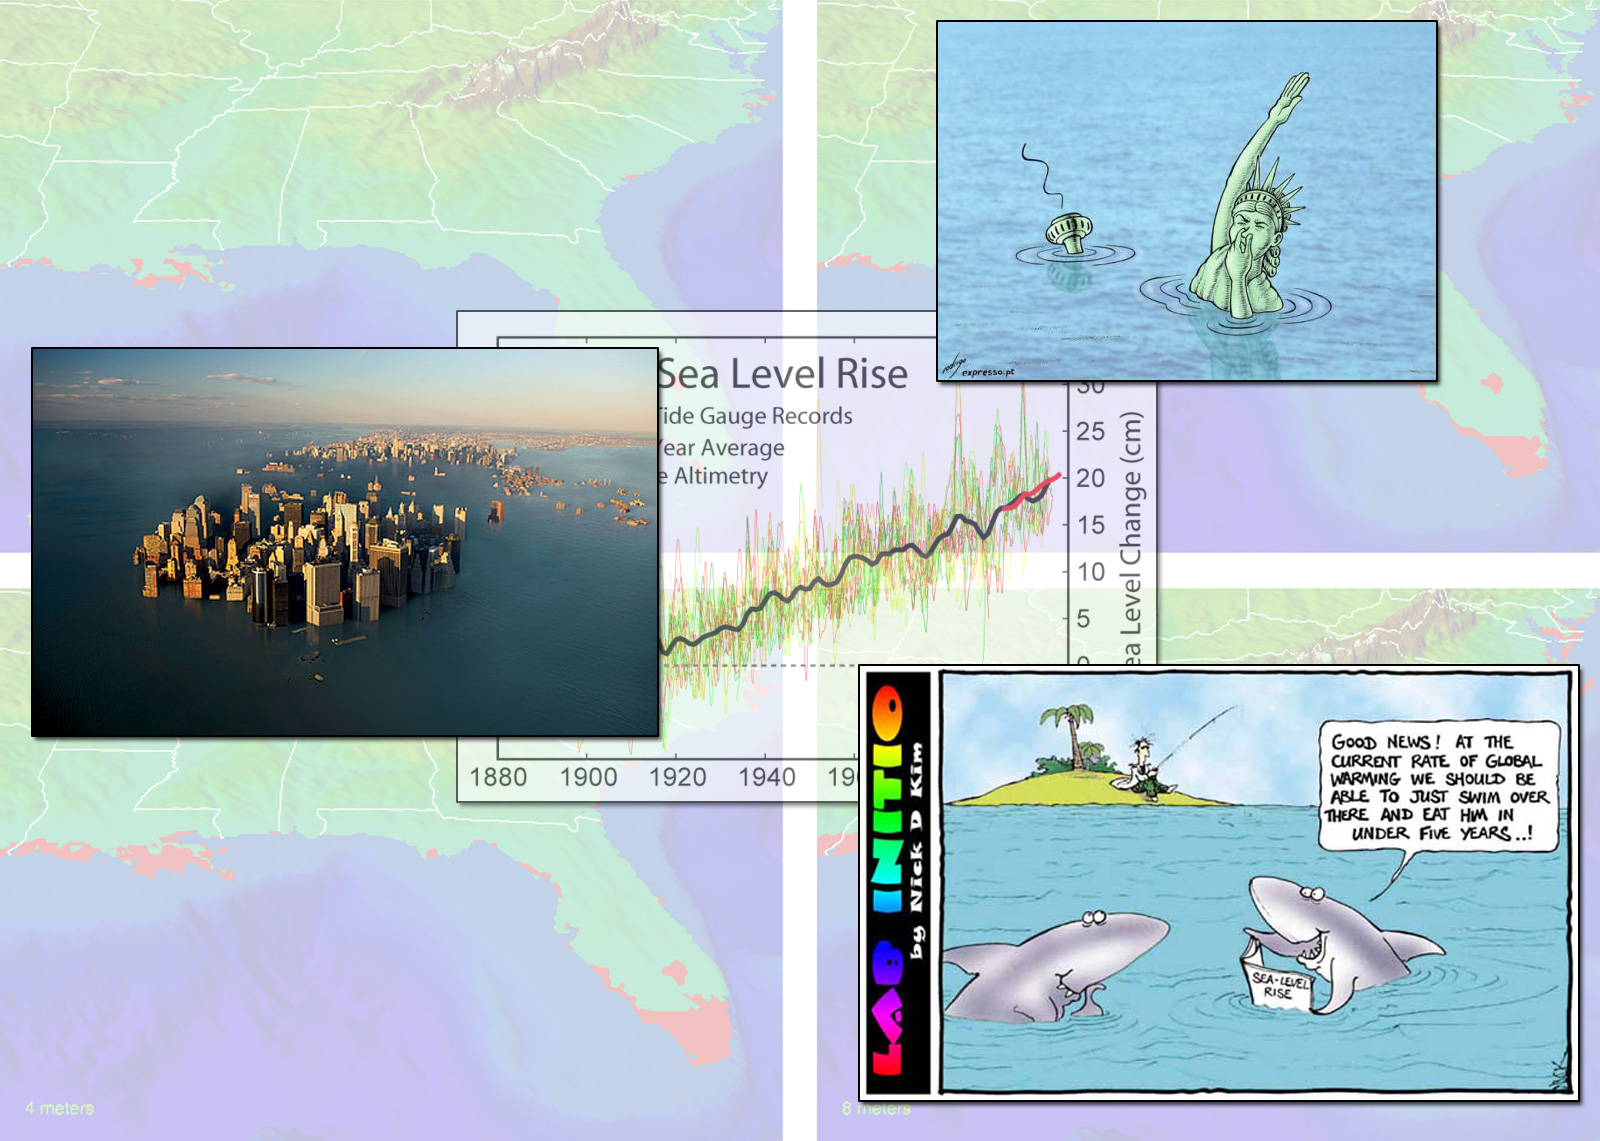
\includegraphics[height=\paperheight,width=\paperwidth]{sea_level_rise_composite}};}
} 

\begin{frame}{How realistic is all this?}
  \note[item]{What can we expect in the next century?}
  \note[item]{In recent years climate scientists and glaciologists}
  \note[item]{have gained a pretty good understanding of what rising air temperatures will}
  \note[item]{In the remainder of the time, I would like to show you some of my own researchl}
\end{frame}


\setbeamertemplate{background canvas}
  {
     \tikz{\node[inner sep=0pt,opacity=0.5] {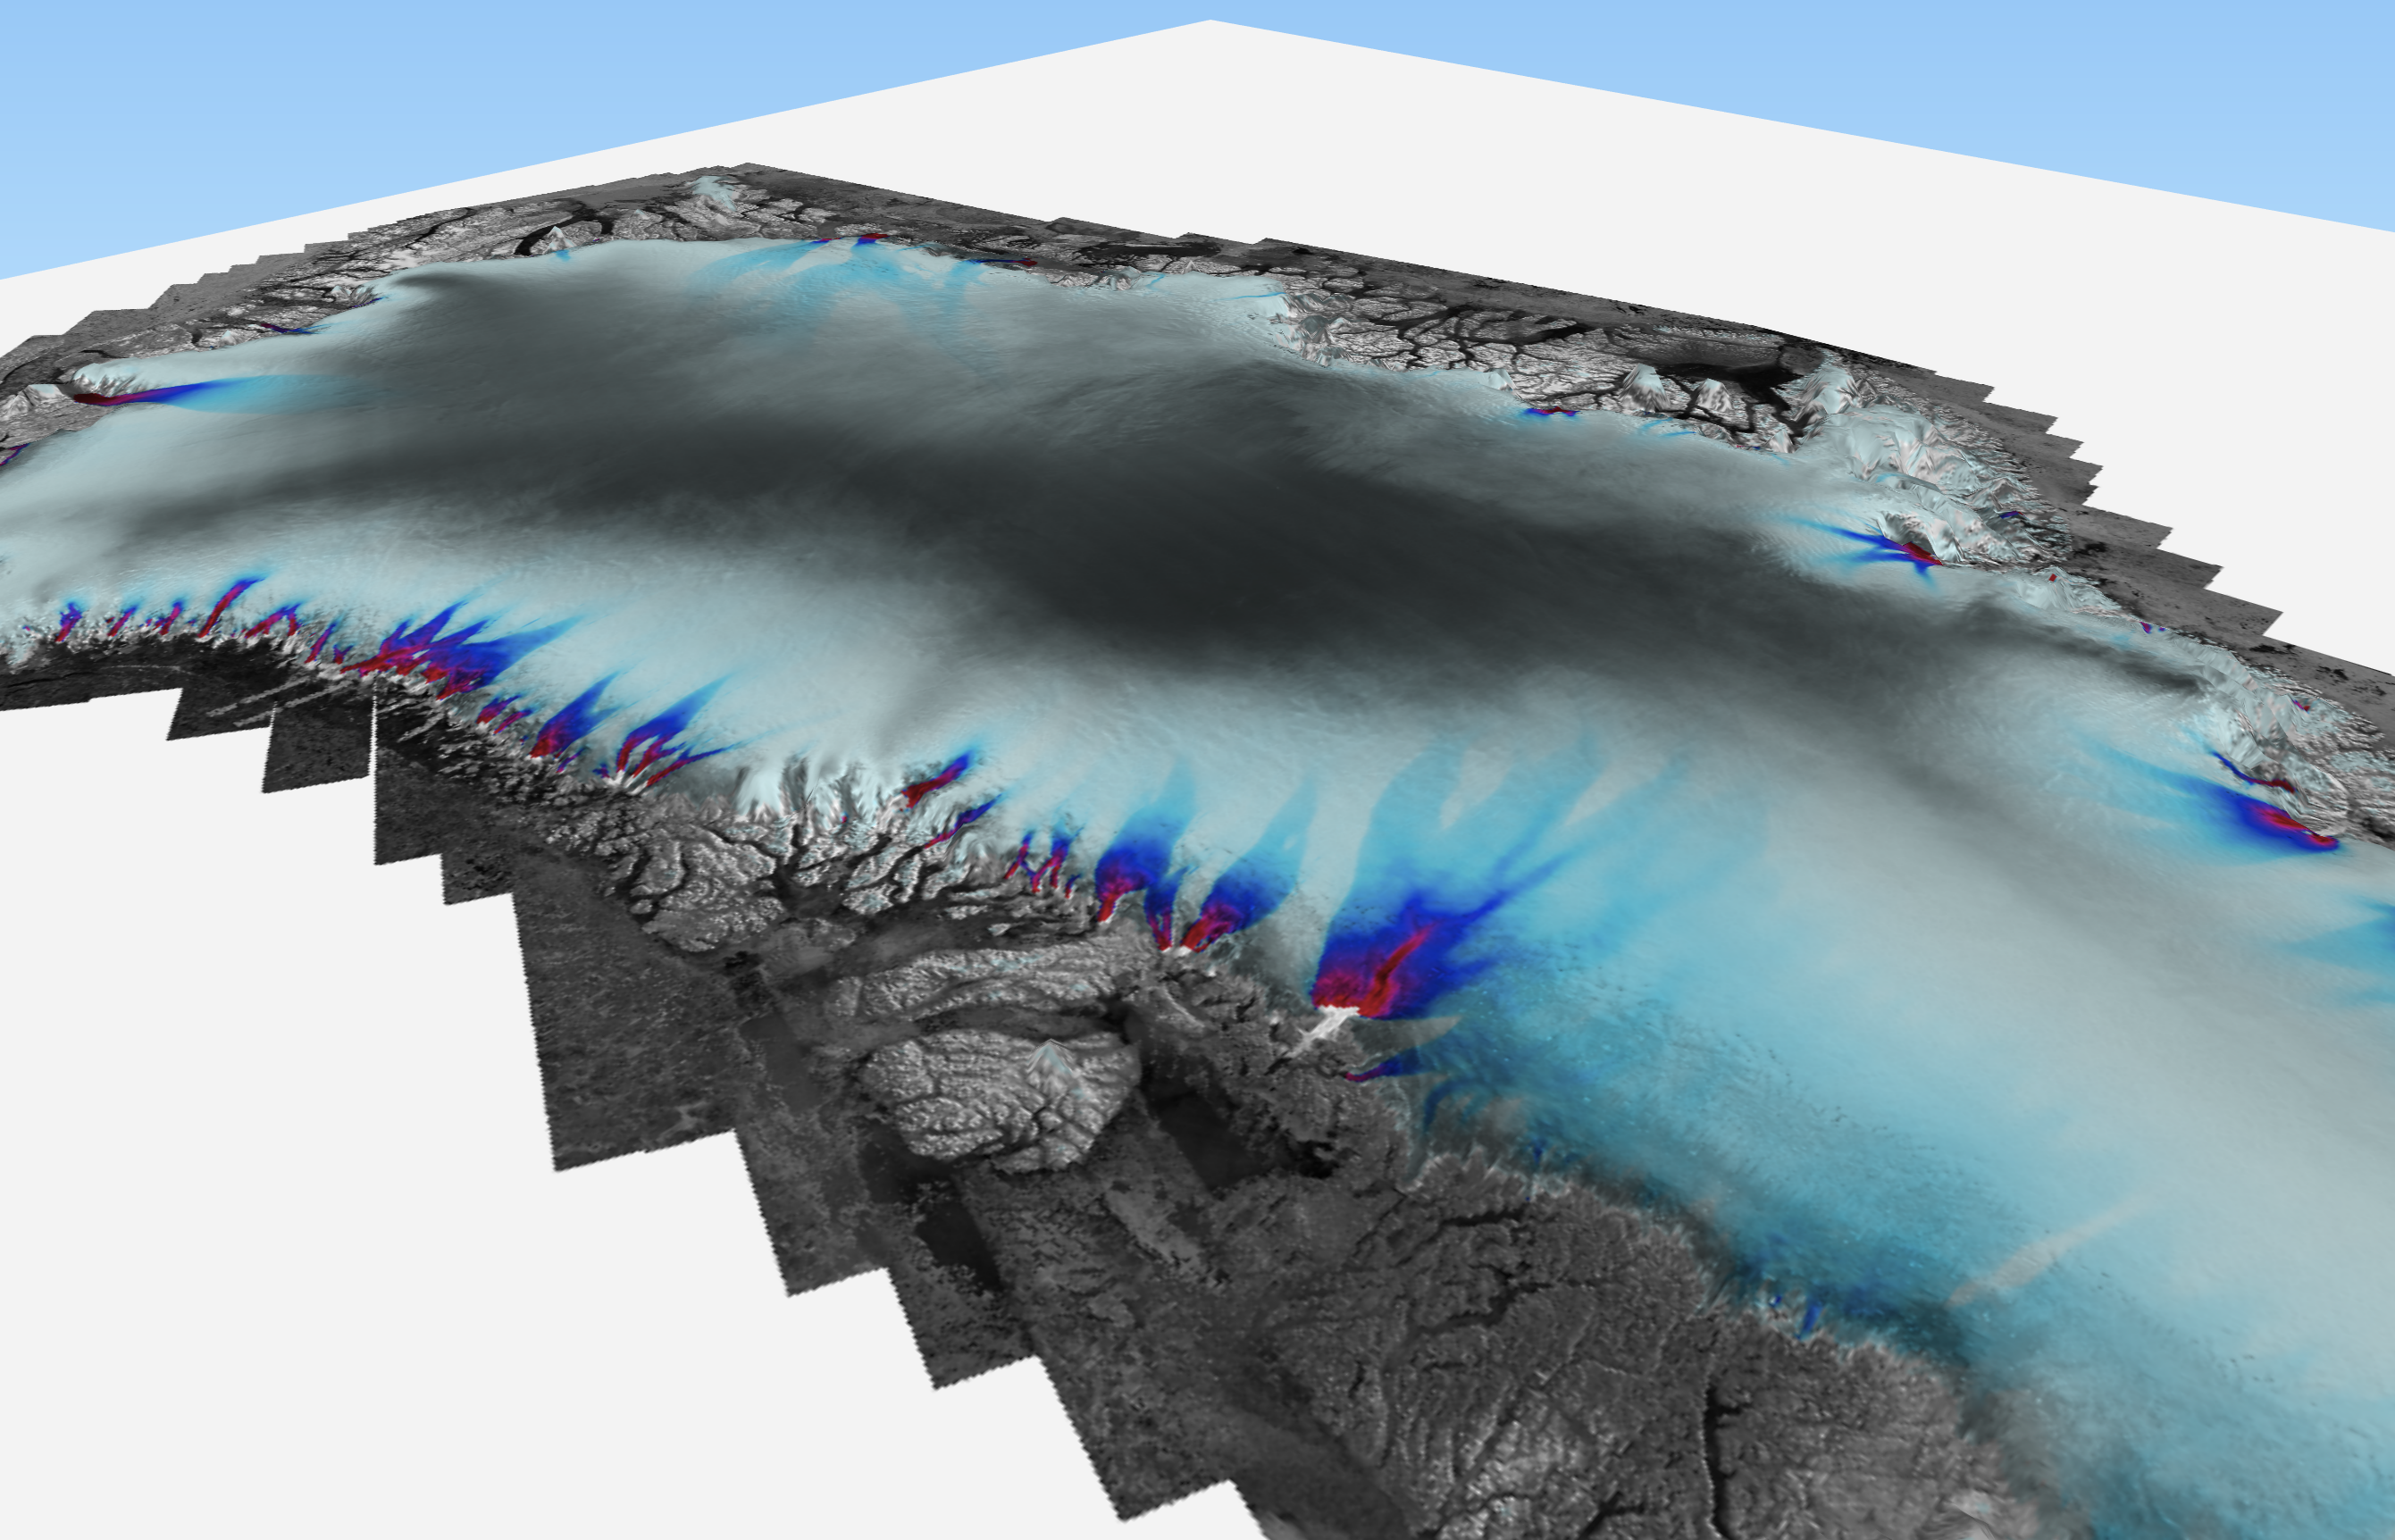
\includegraphics[height=\paperheight,width=\paperwidth]{gris-flow-3d}};}
} 

\begin{frame}{The Parallel Ice Sheet Model}
\begin{transbox}[0.5]
  \begin{figure}
    
\includegraphics[width=0.5\textwidth]{pism-logo}
  \end{figure}
  \begin{itemize}
  \item developed at 
\includegraphics[height=0.5cm]{logo_uaf} since 2007
  \item but legacy code dates back to the 1990s
  \item $>$20 users around the world
  \end{itemize}
\end{transbox}
\end{frame}

\setbeamertemplate{background canvas}
  {
} 

\begin{frame}{Current Applications}
  \begin{figure}
    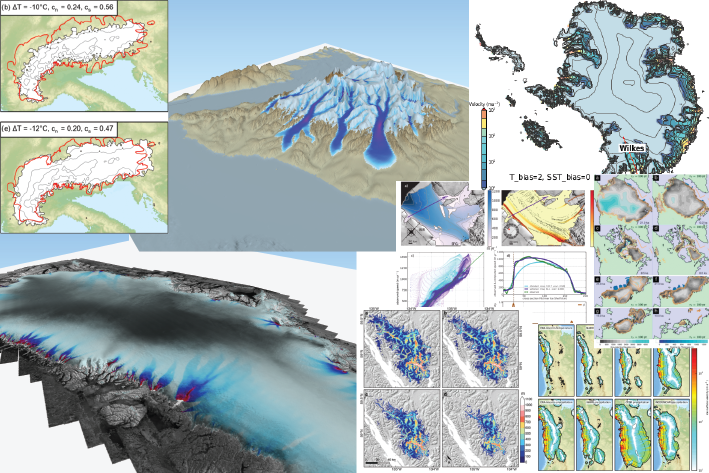
\includegraphics[width=0.9\textwidth]{pism-applications-composite-01}
  \end{figure}
  \note[item]{Lots of different applications}
  \note[item]{In the remainder I'm going to highlight my recent research}
\end{frame}

\setbeamertemplate{background canvas}
  {
     \tikz{\node[inner sep=0pt,opacity=1] {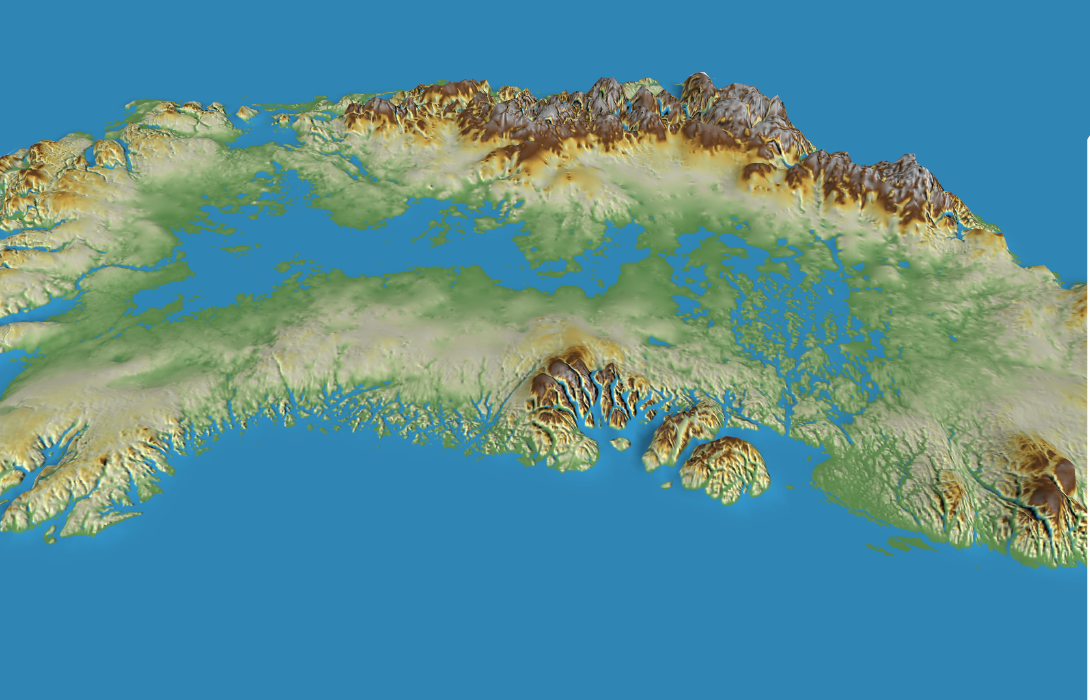
\includegraphics[height=\paperheight,width=\paperwidth]{gris-green-collage-clean}};}
} 

\begin{frame}[plain]
  \note[item]{We know Greenland was nearly ice-free for extended periods during the Pleistocene}
  \note[item]{that's from 2.6 million years ago to 11,700 years ago}
  \note[item]{Maybe Greenland looked somehting like this}
\end{frame}

\setbeamertemplate{background canvas}
  {
     \tikz{\node[inner sep=0pt,opacity=1] {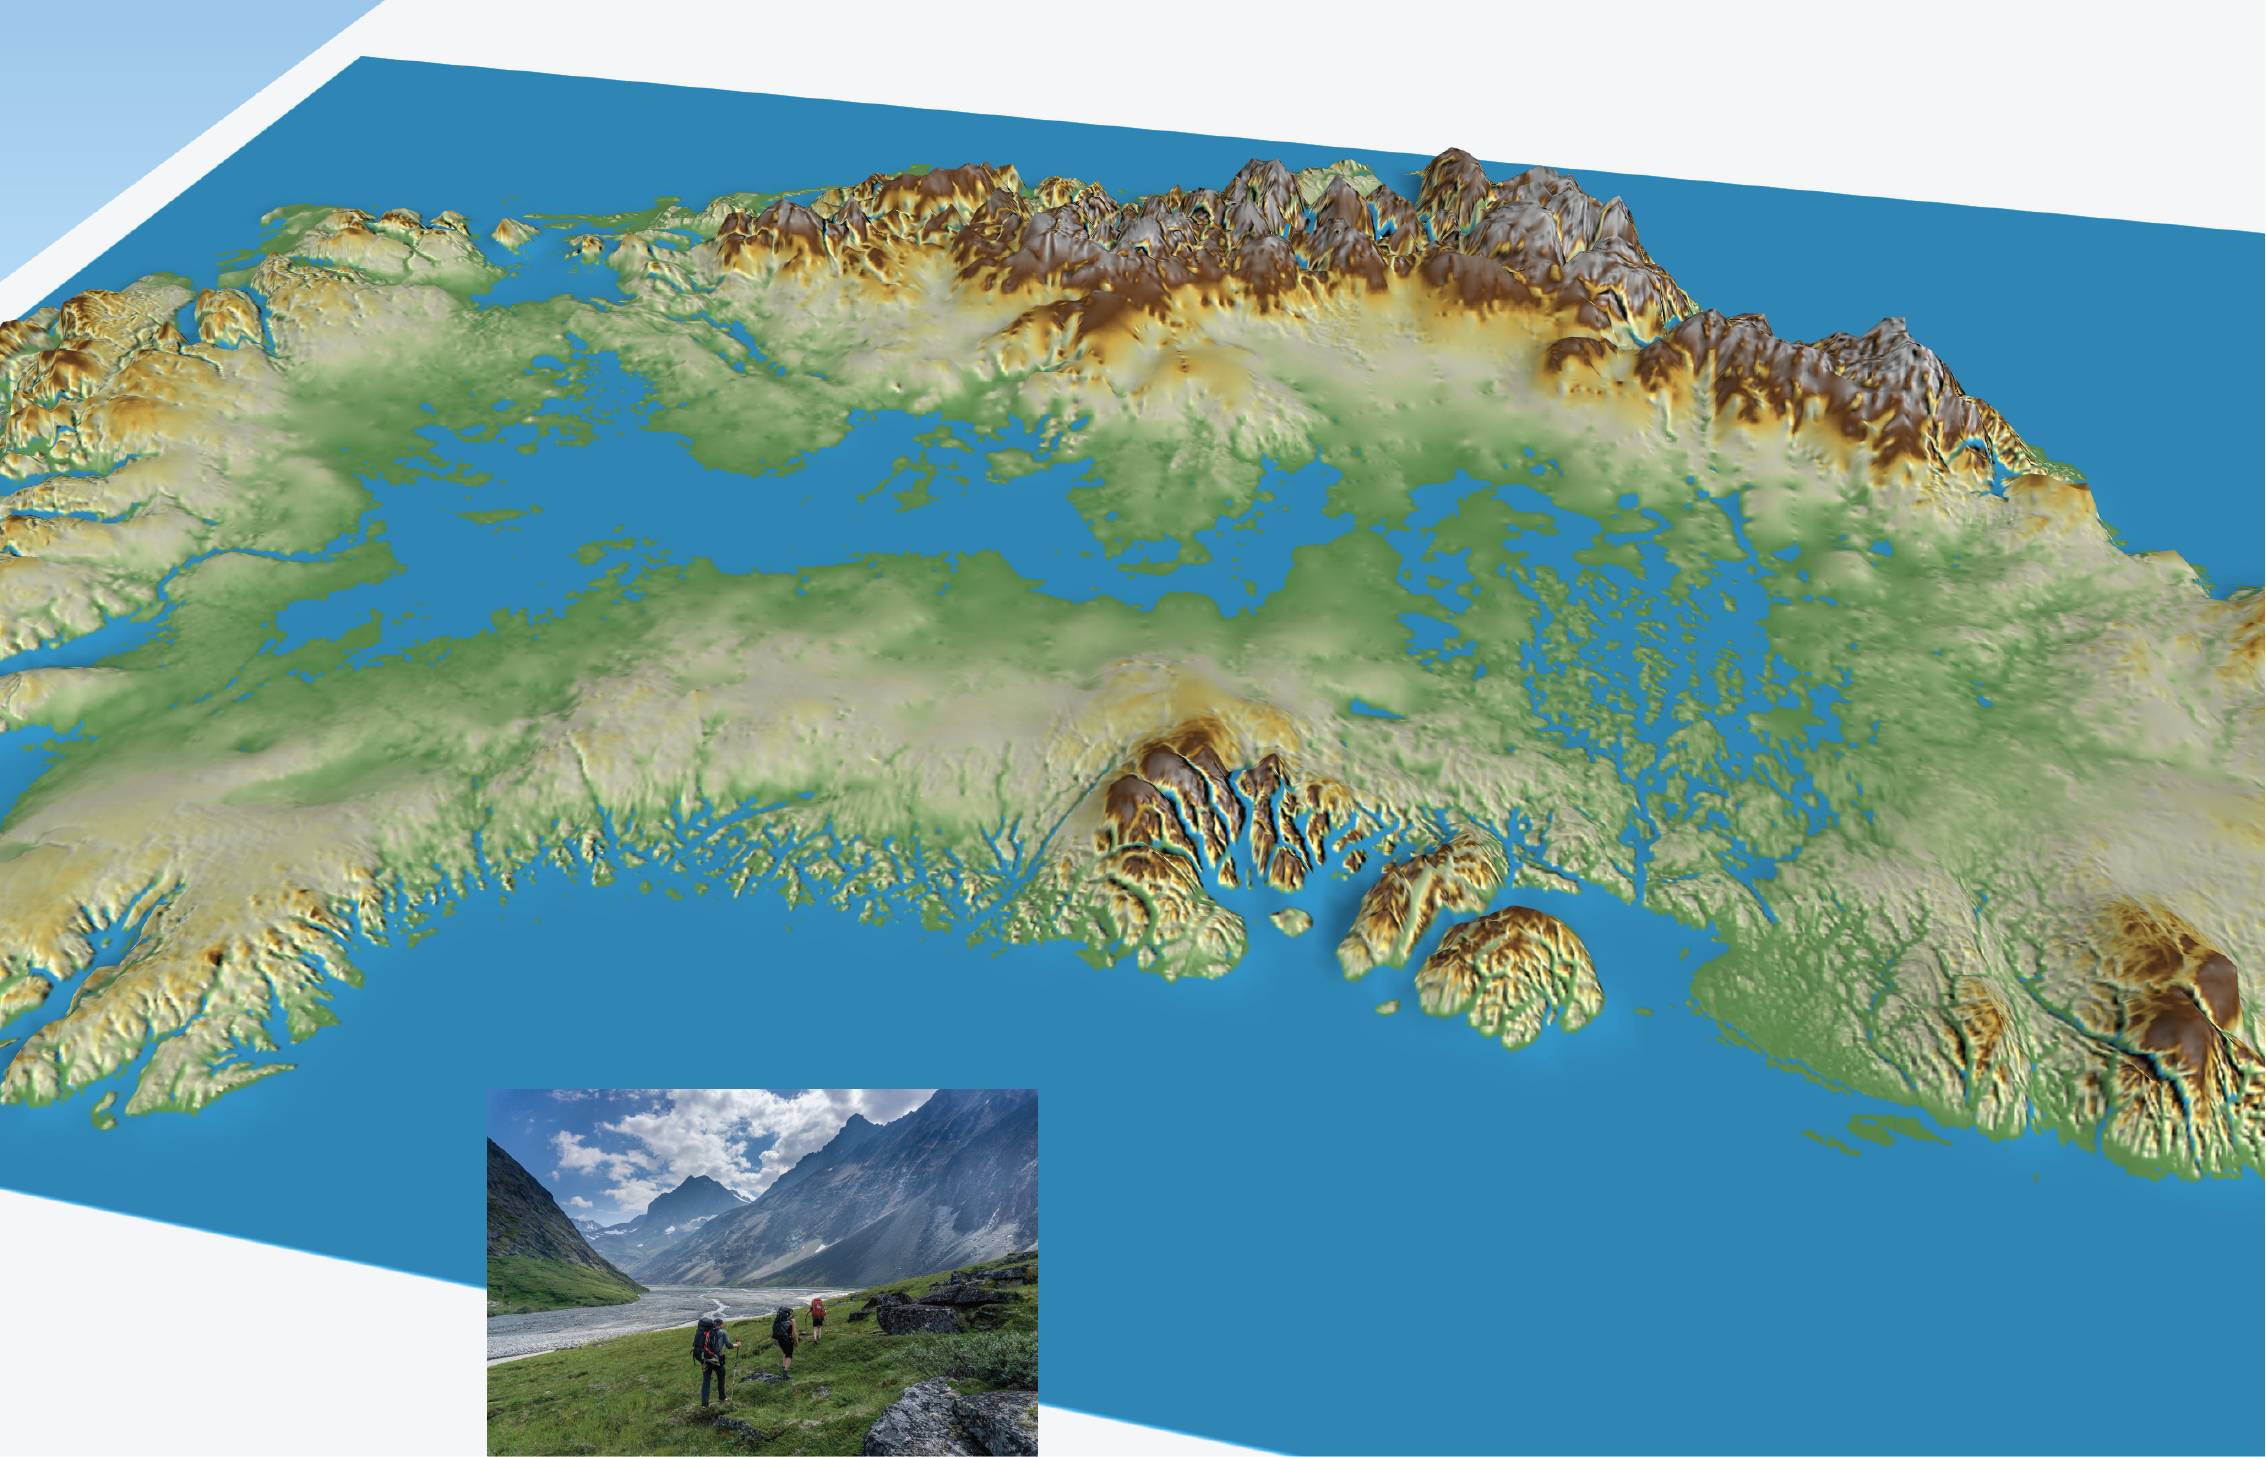
\includegraphics[height=\paperheight,width=\paperwidth]{gris-green-collage-1}};}
} 

\begin{frame}[plain]
  \note[item]{Lots of space to go hiking}
\end{frame}

\setbeamertemplate{background canvas}
  {
     \tikz{\node[inner sep=0pt,opacity=1] {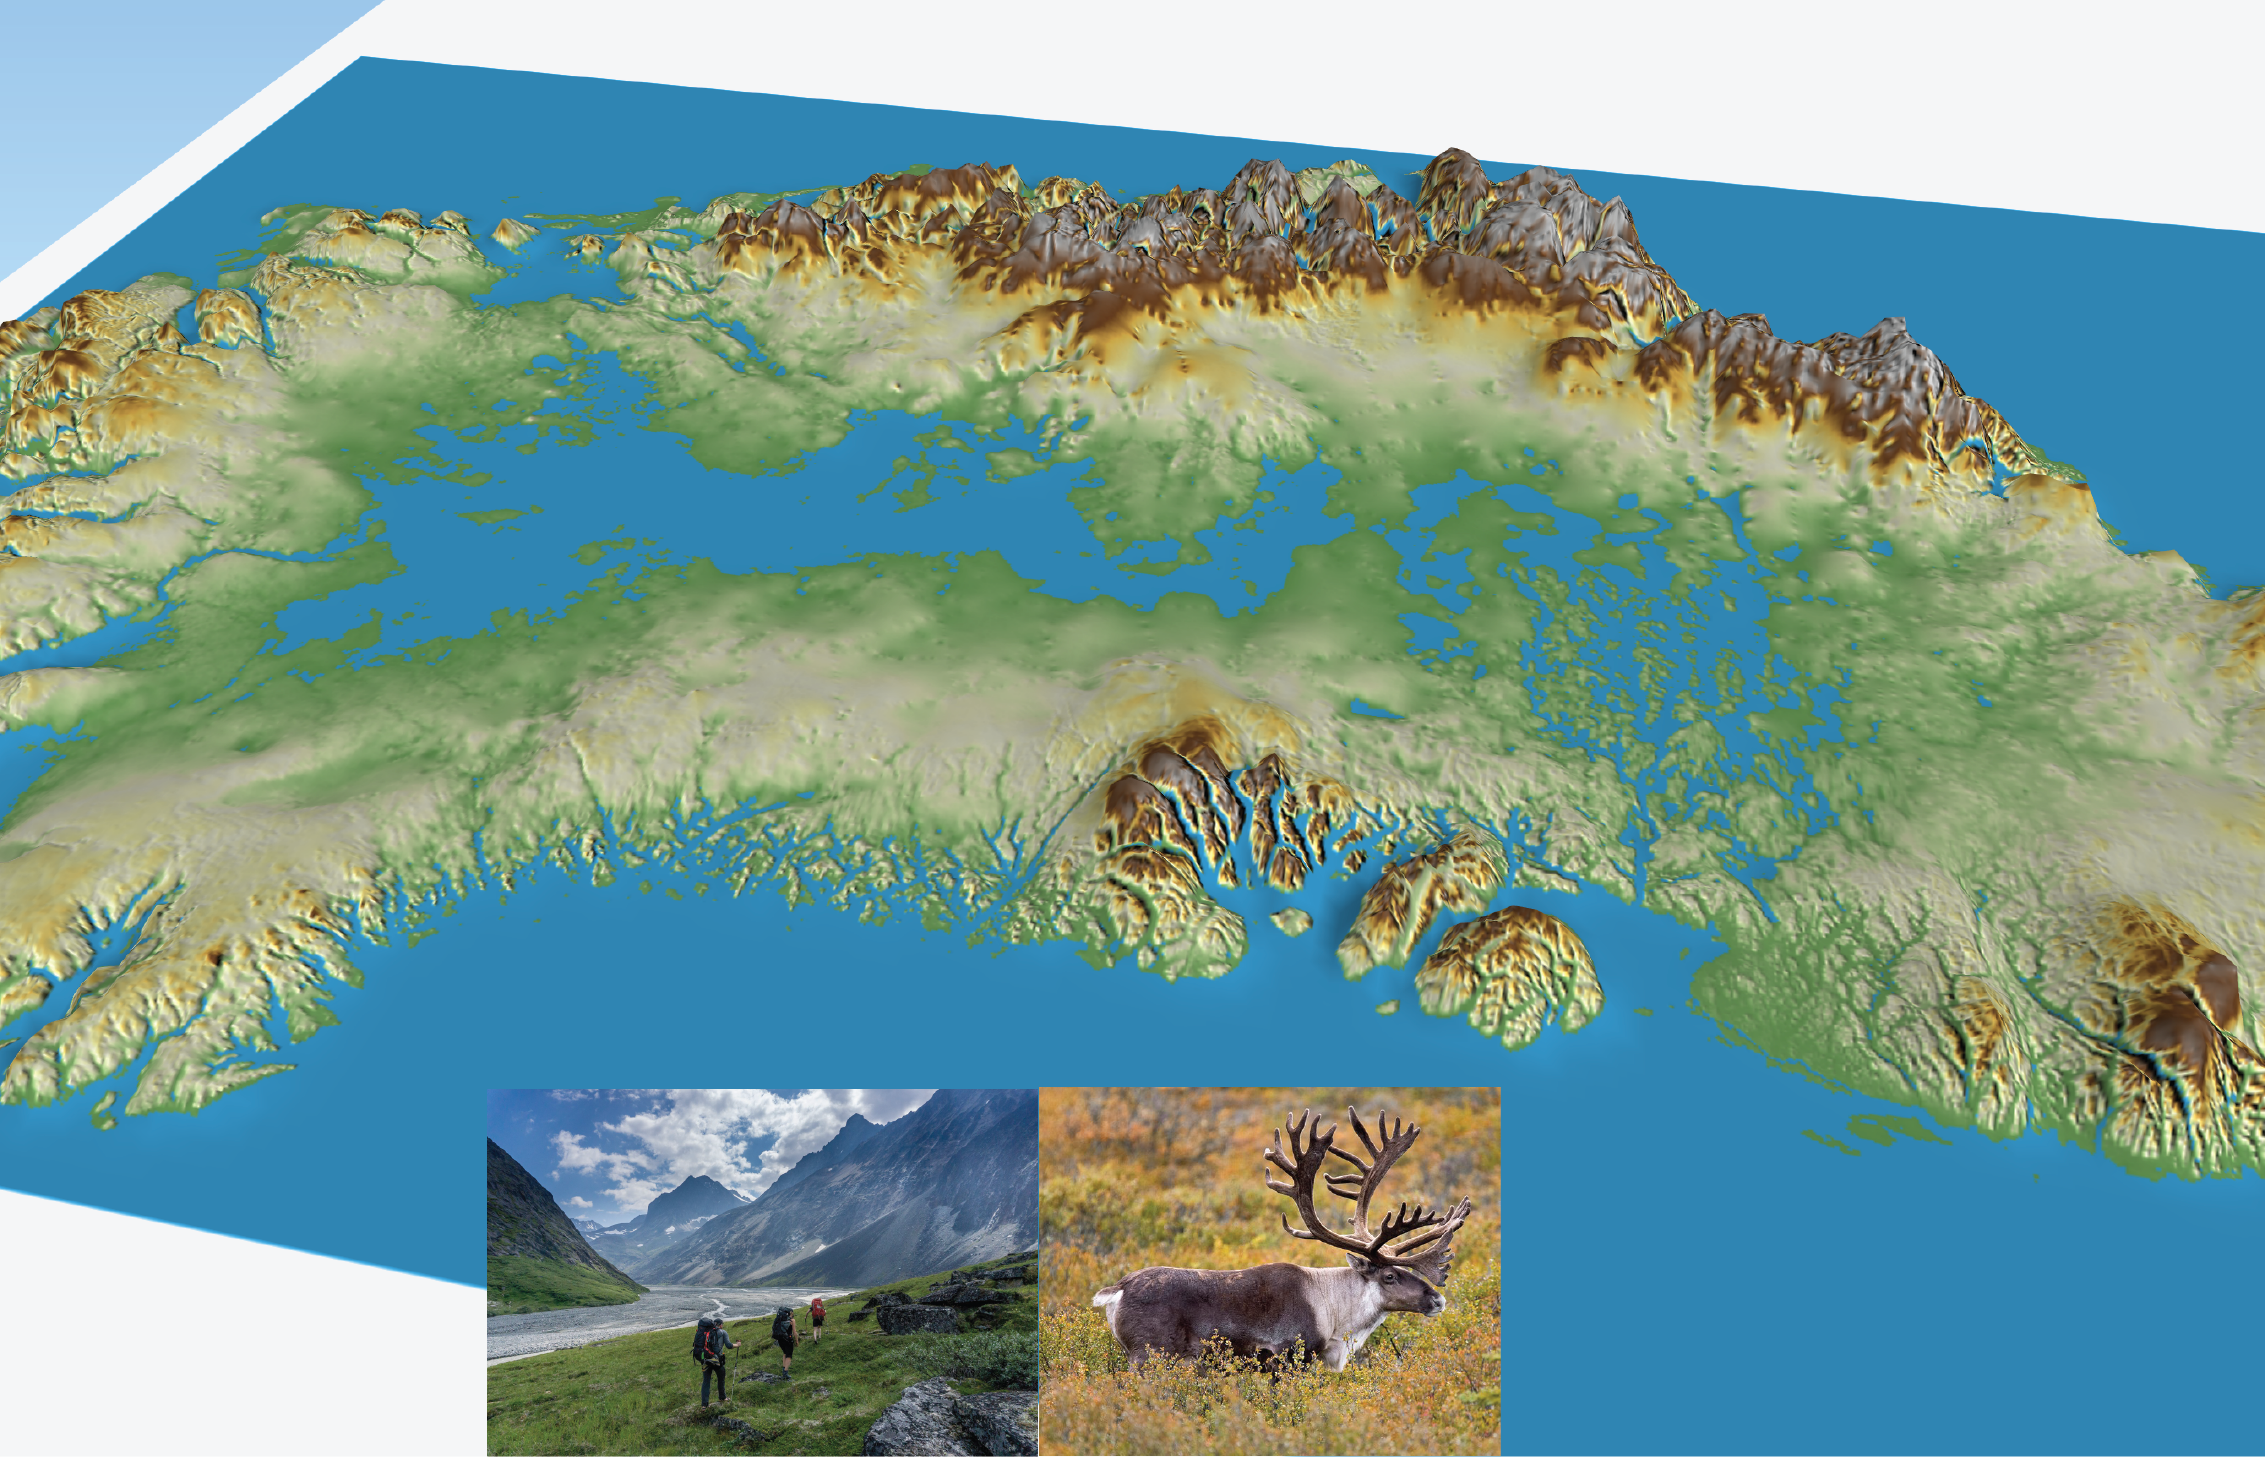
\includegraphics[height=\paperheight,width=\paperwidth]{gris-green-collage-2}};}
} 

\begin{frame}[plain]
  \note[item]{For caribous to roam}
\end{frame}

\setbeamertemplate{background canvas}
  {
     \tikz{\node[inner sep=0pt,opacity=1] {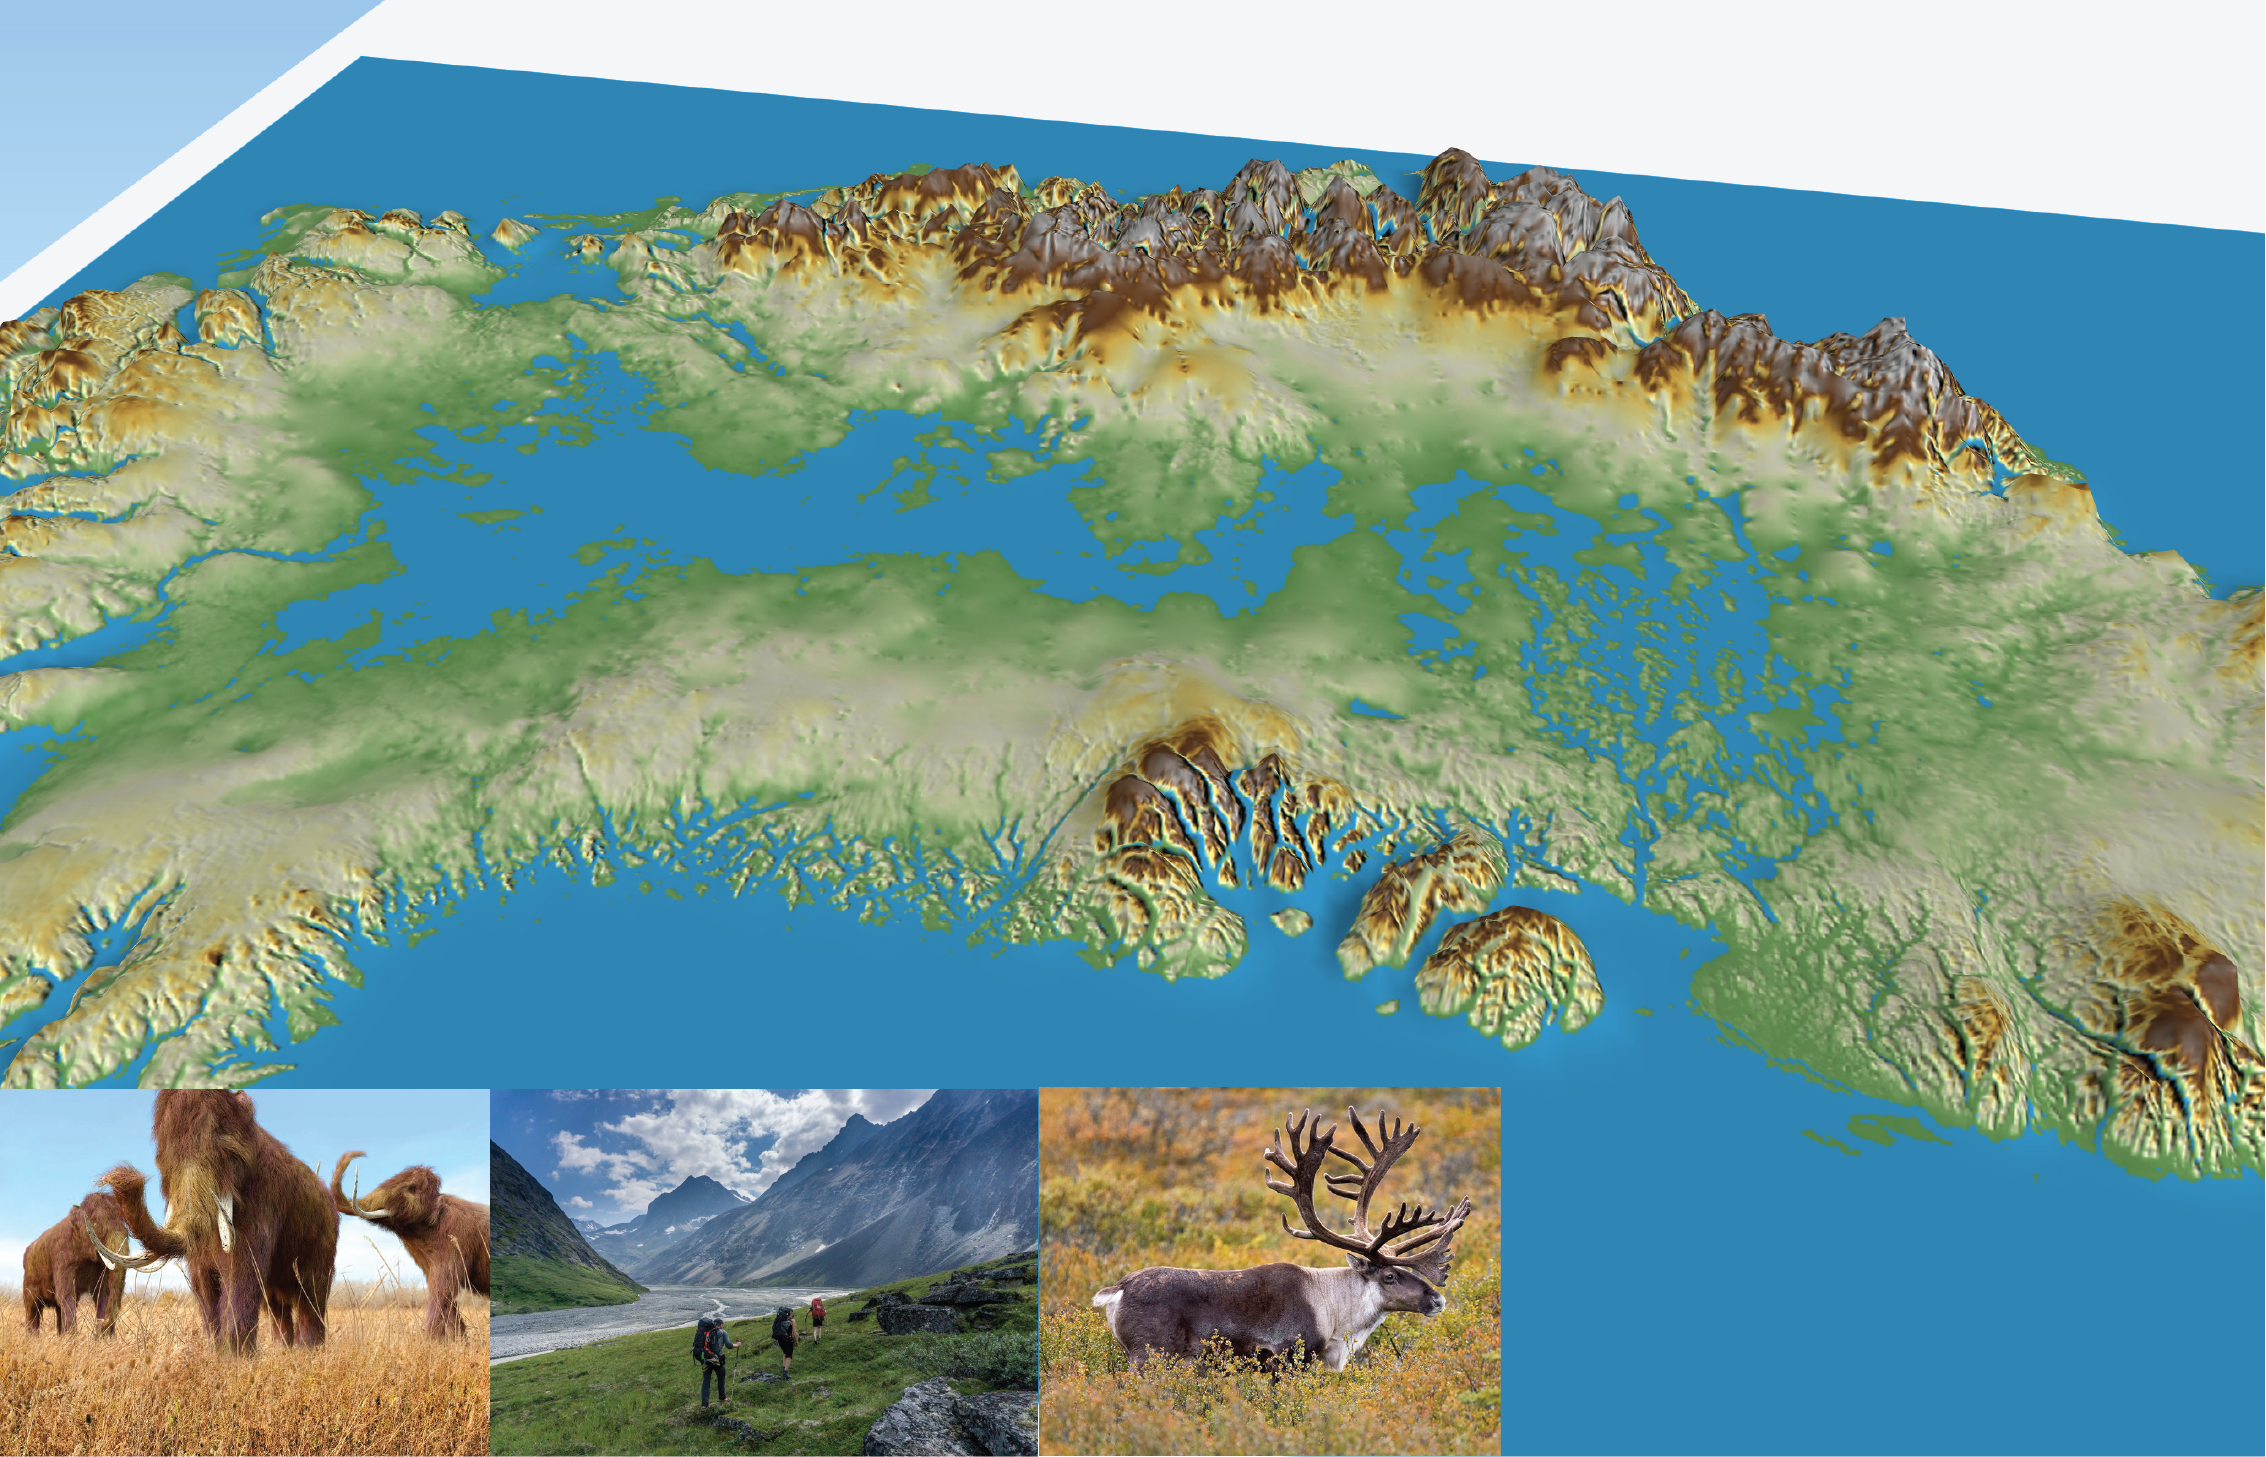
\includegraphics[height=\paperheight,width=\paperwidth]{gris-green-collage-3}};}
} 

\begin{frame}[plain]
  \note[item]{or like a Jurassic Park}
  \note[item]{Now the interesting question is:}
  \note[item]{Can this happen again}
  \note[item]{and under what conditions?}

\end{frame}


\setbeamertemplate{background canvas}
{
%
}


\begin{frame}{Observed vs simulated flow speeds in 1999}
  \begin{columns}[c]
    \begin{column}{.65\linewidth}
      \begin{figure}
        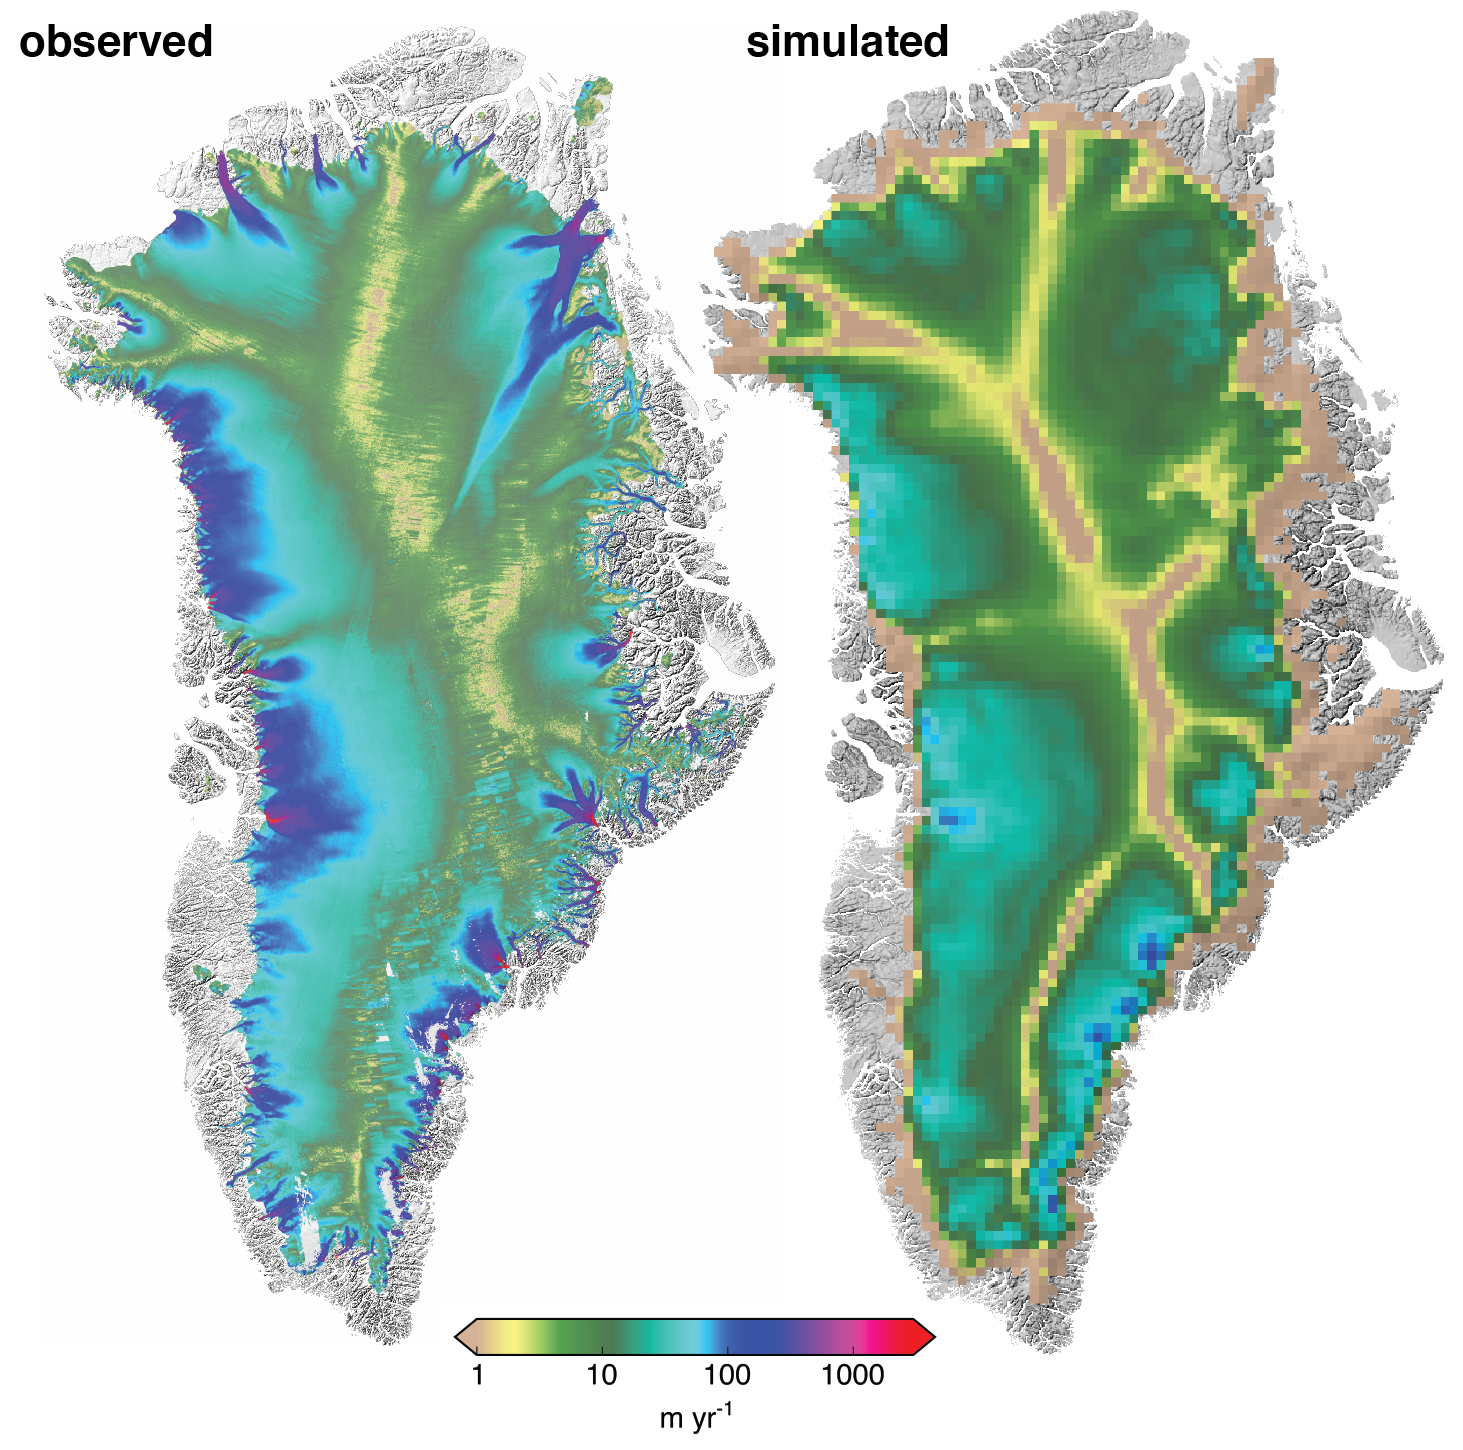
\includegraphics[width=\textwidth]{gris-obs-exp-old-1999}
      \end{figure}
    \end{column}
    \begin{column}{.35\linewidth}
      \begin{block}{Roadblock}
        \begin{figure}
          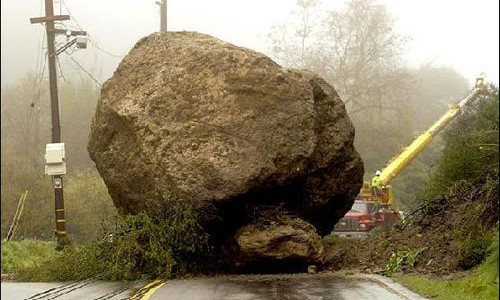
\includegraphics[width=\textwidth]{roadblocks}
        \end{figure}
        \begin{itemize}
        \item can't reproduce flow field
        \end{itemize}
      \end{block}
    \end{column}
  \end{columns}
  \note[item]{ISM were excluded from AR4}
  \note[item]{Explain colorbar}
  \note[item]{Explain plots}
\end{frame}

\begin{frame}{Observed vs simulated flow speeds in 2013}
  \begin{columns}[c]
    \begin{column}{.65\linewidth}
      \begin{figure}
        \includegraphics[width=\textwidth]{gris-obs-exp-old}
      \end{figure}
    \end{column}
    \begin{column}{.35\linewidth}
      \begin{block}{Roadblock}
        \begin{figure}
          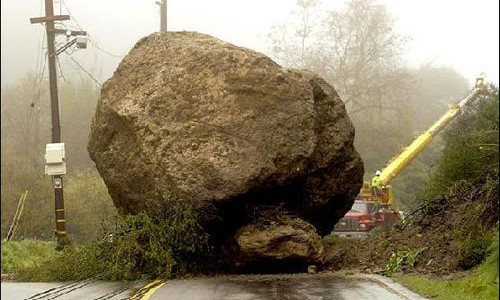
\includegraphics[width=\textwidth]{roadblocks}
        \end{figure}
        \begin{itemize}
        \item a bit better than in 1999
        \item but still can't reproduce flow field
        \end{itemize}
      \end{block}
    \end{column}
  \end{columns}
  \note[item]{Some improvement}
\end{frame}


\begin{frame}{Ice thickness and simulated flow speeds}
\vspace{-0.74em}
  \begin{columns}
    \column[c]{5cm}
    \begin{figure}
      \includegraphics<1-2>[width=\textwidth]{greenland-obs-basal-overview}
      \includegraphics<3-4>[width=\textwidth]{greenland-obs-basal-overview-mo14}
    \end{figure}
    \column[c]{5cm}
    \only<1,3>{Jakobshavn Isbr{\ae}}
    \only<2>{no fast flow}
    \only<4>{fast flow appears}
    \includegraphics<1>[width=\textwidth]{jakobshavn-bed-5000m-ba01}
    \includegraphics<2>[width=\textwidth]{jakobshavn-speed-exp-4500m-ba01}
    \includegraphics<3>[width=\textwidth]{jakobshavn-bed-mo14}
    \includegraphics<4>[width=\textwidth]{jakobshavn-speed-exp-600-v1.2-no-scale-no-gate}
    \only<1>{\\ 5\,km, old data set (2001)}
    \only<2,4>{\\ simulated surface speed}
    \only<3>{\\ 600\,m, new data set (2014)}
  \end{columns}
  \note<1>[item]{now let's do a simualulation with the old ice thickness data}
  \note<2>[item]{there isn't really any fast flow}
  \note<3>[item]{now use the new ice thickness}
  \note<4>[item]{and we get fast flow}
\end{frame}


\begin{frame}{We can capture the present-day flow field}
  \begin{figure}
    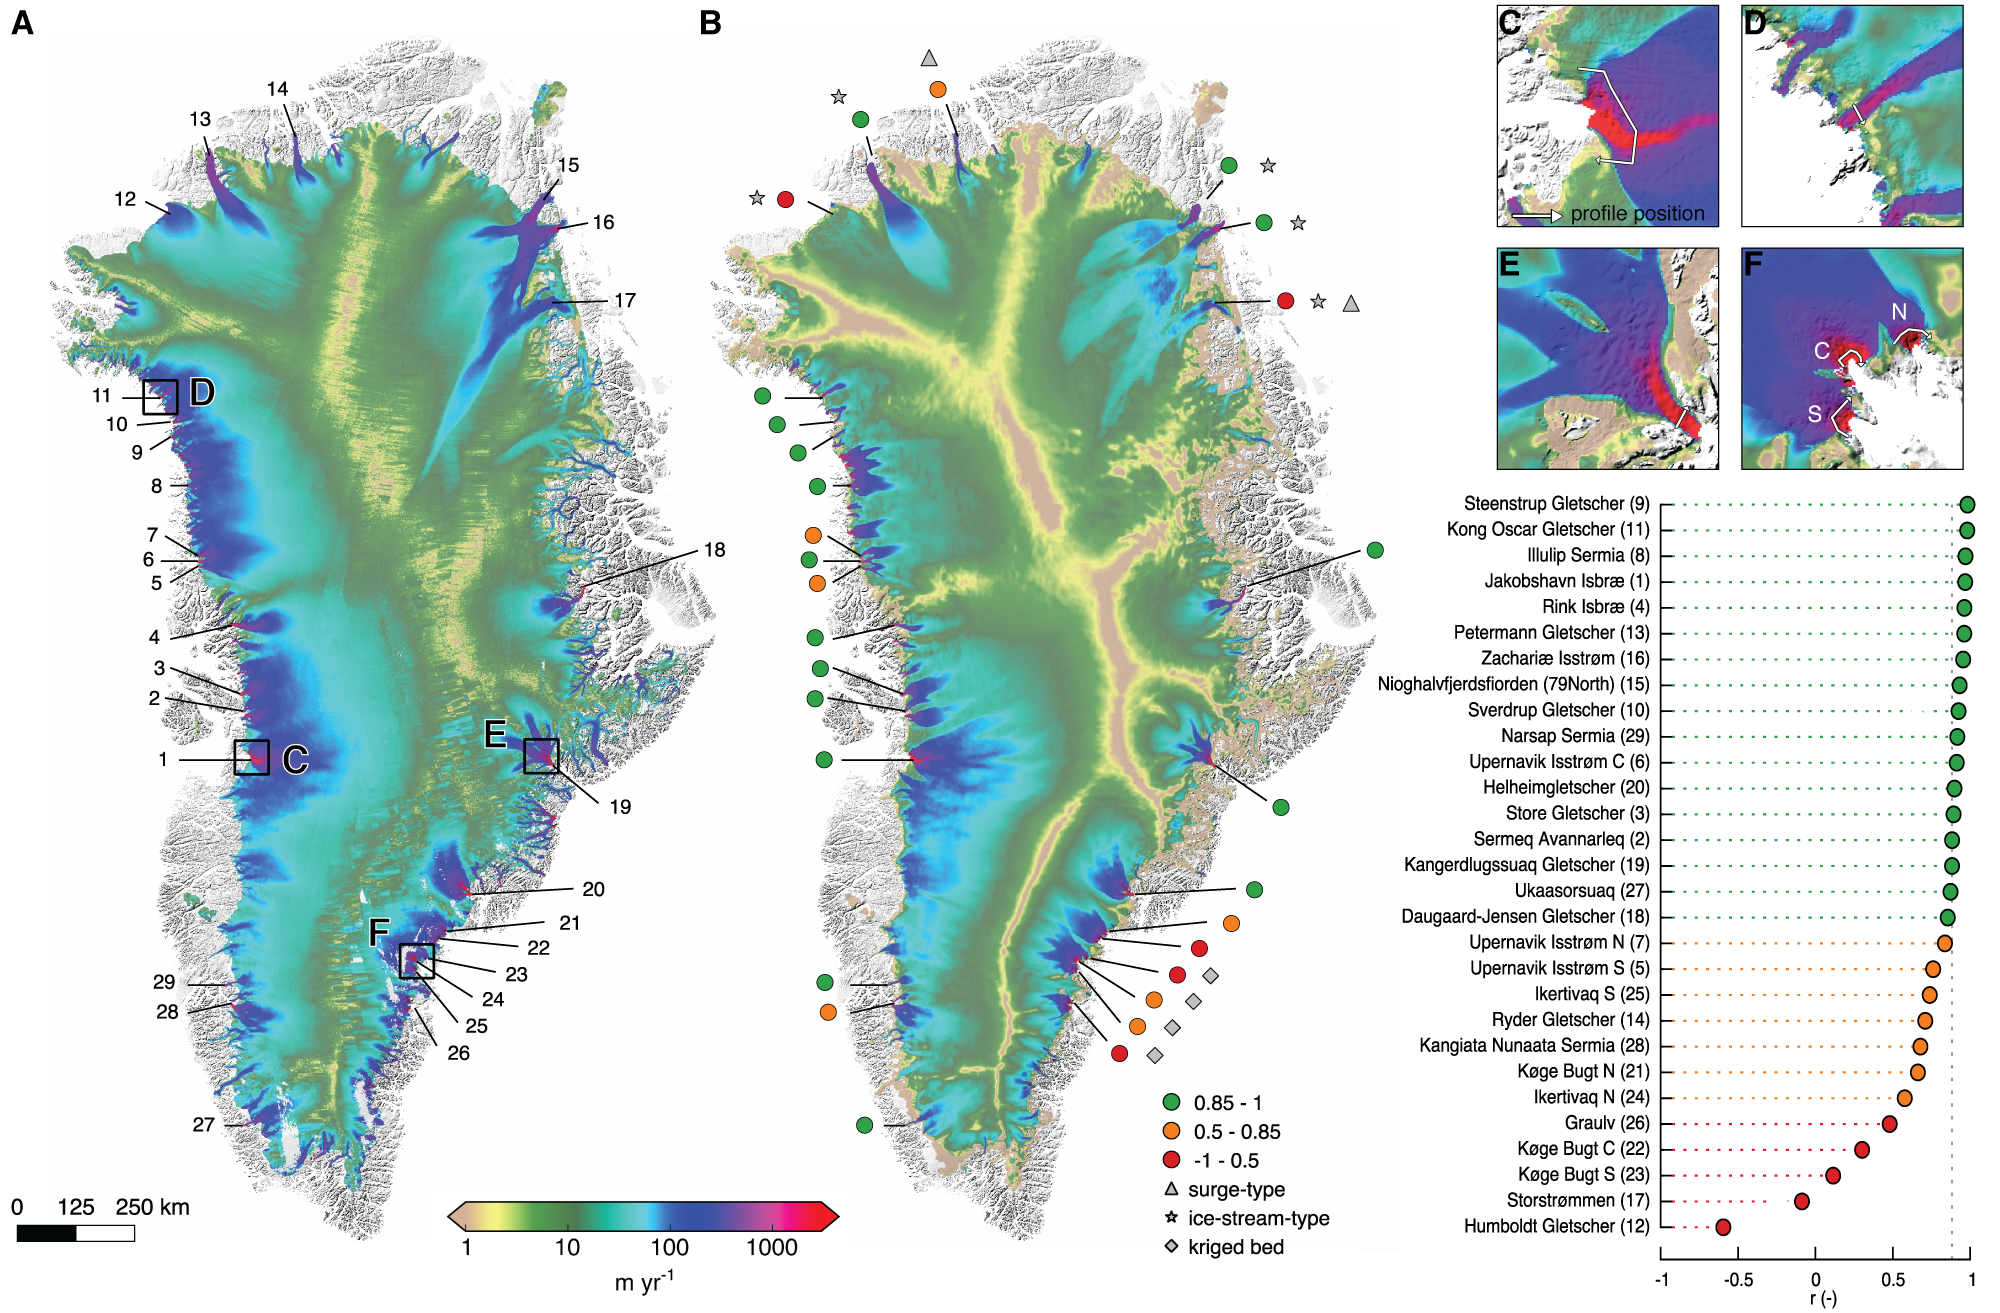
\includegraphics[height=7cm]{greenland-overview-3}
    \\ \scriptsize{Aschwanden, Fahnestock, Truffer (2016) \textit{Nature Communications}}
  \end{figure}
  \note[item]{first time capturing the flow field for the right reason}
  \note[item]{this is quite a break through in ice sheet modeling}
  \note[item]{though not a surprising one}
  \note[item]{it just confirms what students learn in glaciology 100:}
  \note[item]{ice flows downhill}
\end{frame}

\begin{frame}{Ready for a new assessment}
  \begin{figure}
    \includegraphics[width=11cm]{gris-pism-setup-2018}
  \end{figure}
  \note[item]{Over the past year, we've assembled the best data sets}
  \note[item]{added new model physics such better calving parameterizations}
  \note[item]{to bring you the first post-AR5 sea level estimates}
  \note[item]{for the next millennium}
  \note[item]{\alert{that resolve outlet glaciers}}
\end{frame}

\begin{frame}
  \frametitle{Evolution over the next millennium}
  \begin{columns}[c]
    \begin{column}{.85\linewidth}
      \begin{figure}
        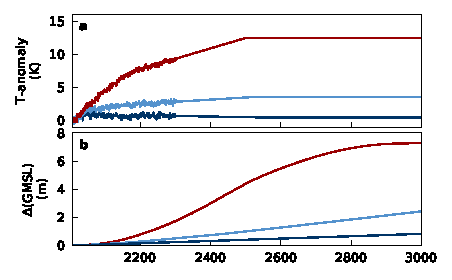
\includegraphics[width=\textwidth]{les18_ctrl}
      \end{figure}
    \end{column}
    \begin{column}{.15\linewidth}
      \begin{figure}
        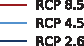
\includegraphics[height=1cm]{legend-rcp}
      \end{figure}
    \end{column}
  \end{columns}
  \note[item]{We took three representative concentration pathway (RCP) scenarios}
  \note[item]{using temperature forcing from a GCM}
  \note[item]{and performed three simulations for a thousand years}
  \note[item]{explain figures and results}
\end{frame}


\begin{frame}
  \frametitle{Uncertainty analysis}
  \begin{columns}[c]
    \begin{column}{.3\linewidth}
    \begin{figure}
    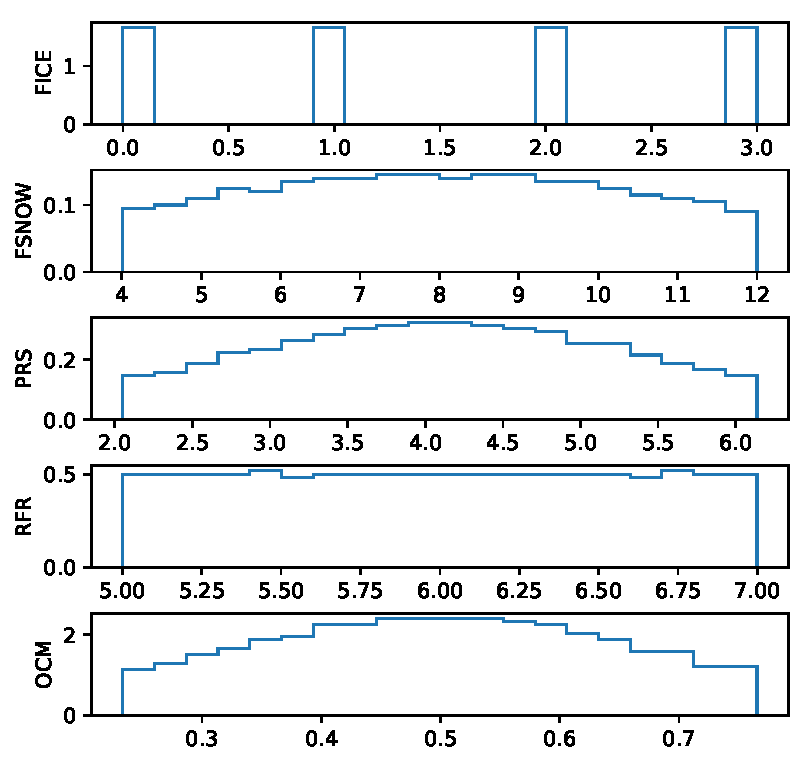
\includegraphics[width=\textwidth]{parameter_histograms}
    \end{figure}
    \end{column}
    \begin{column}{.7\linewidth}
  \begin{itemize}
  \item choose the 4 GCMs and 10 parameters
  \item prescribe distributions (normal, uniform, truncated normal, gamma)
  \item draw 500 samples using Latin Hypercube Sampling
  \item run 500 simulations at 1.8\,km resolution per RCP (1,500 total)
  \item run control simulation at 900\,m resolution (ensemble mean forcing)
  \item Sobel indices attribution analysis
  \item 2M CPU hours
  \end{itemize}
    \end{column}
  \end{columns}
\end{frame}

\begin{frame}
  \frametitle{Evolution over the next millennium}
  \begin{columns}[c]
    \begin{column}{.85\linewidth}
    \begin{figure}
    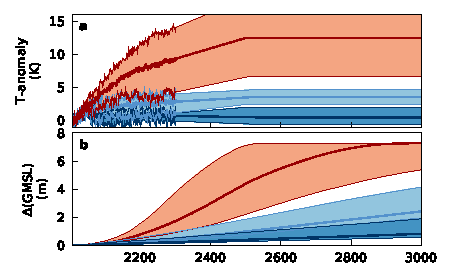
\includegraphics[width=\textwidth]{les18_les}
    \end{figure}
    \end{column}
    \begin{column}{.15\linewidth}
      \begin{figure}
        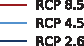
\includegraphics[height=1cm]{legend-rcp}
      \end{figure}
    \end{column}
  \end{columns}
\end{frame}

\begin{frame}
  \frametitle{In a thousand years}
  \begin{figure}
    \includegraphics[height=6.5cm]{rcp-final-states-extend}
  \caption{Likelihood of a pixel being ice covered.}
  \end{figure}
  \note[item]{In a thousand years, Greenland will look different to today}
  \note[item]{Explain uncertainty map}

\end{frame}

\begin{frame}[plain]
  \begin{figure}
  \includemedia[
  width=8cm,
  activate=pageopen,
  addresource=gris-g900m_rcps-hd1920.mov,
  flashvars={source=gris-g900m_rcps-hd1920.mov
    &modestbranding=1 % no YT logo in control bar
    &autohide=0
    &showinfo=0
    &rel=0
    % controlbar autohide
    % no title and other info before start
    % no related videos after end
  }
  ]
  {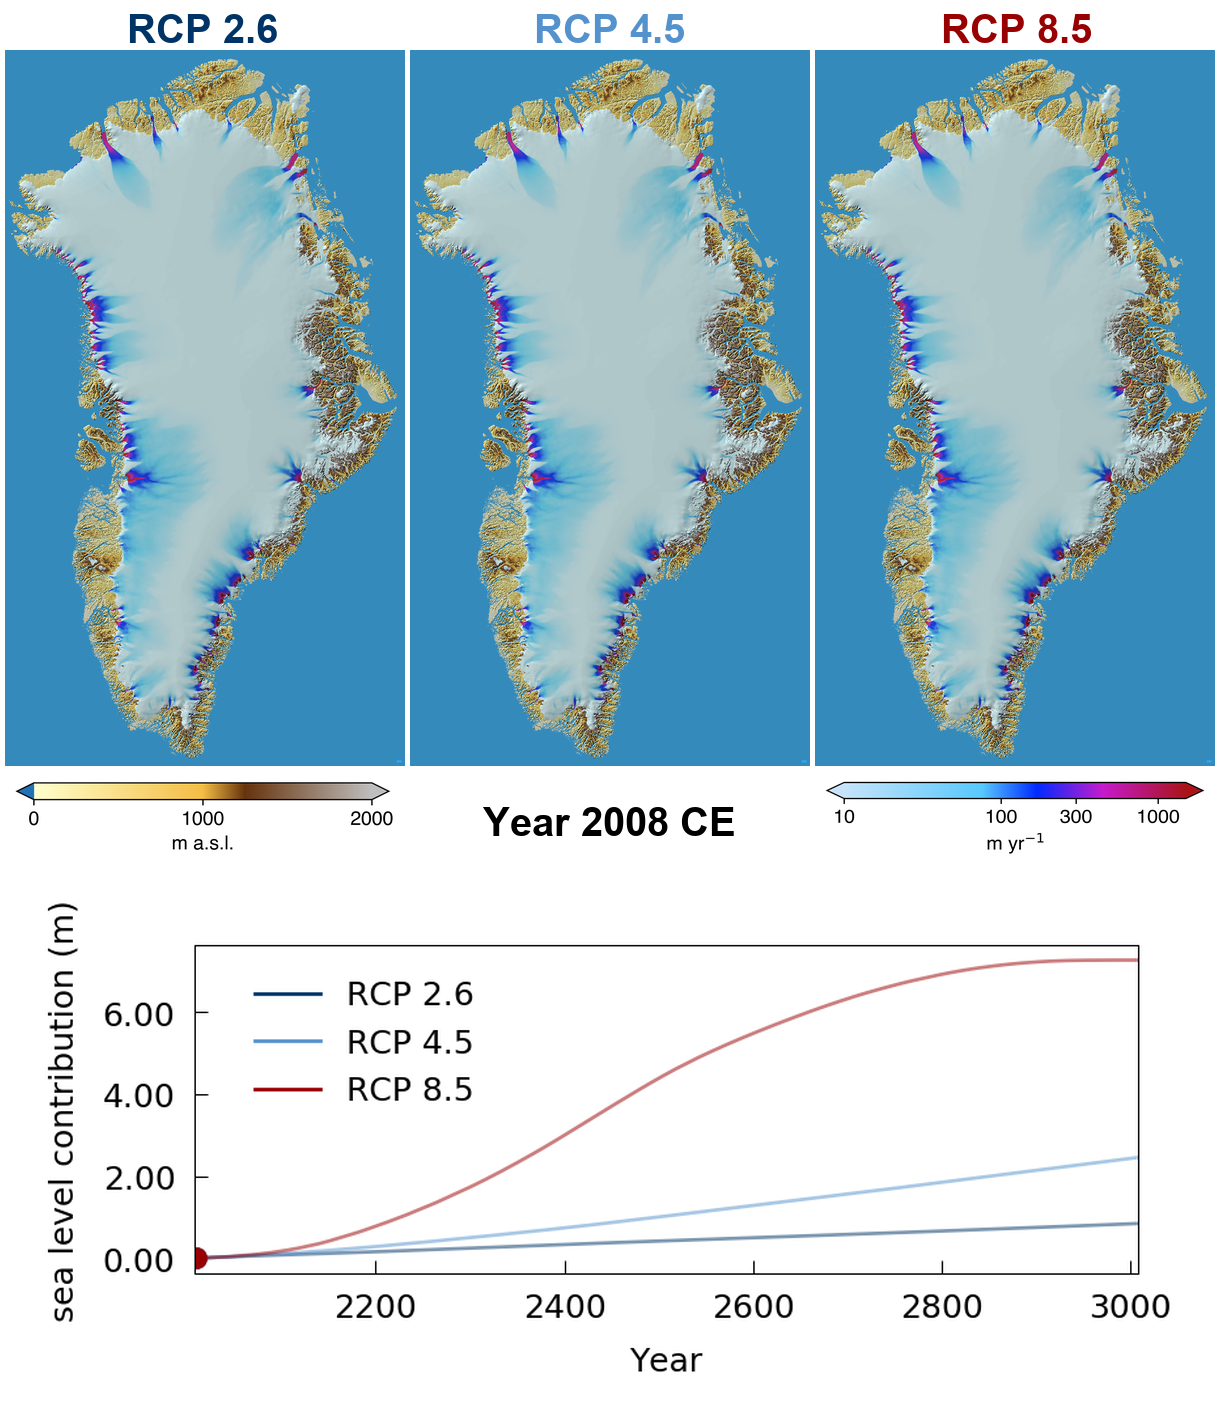
\includegraphics[width=8cm]{gris_g900m_rcps_0000}}{VPlayer.swf}
\end{figure}
\end{frame}


\begin{frame}
  \frametitle{Outlet glacier retreat}
  \begin{figure}
    \includegraphics<1>[width=\textwidth]{flowline-composite-1gl-uis} 
    \includegraphics<2>[width=\textwidth]{flowline-composite-1gl-sg} 
  \end{figure}
\end{frame}




\setbeamertemplate{background canvas}
  {
     \tikz{\node[inner sep=0pt,opacity=1.0] {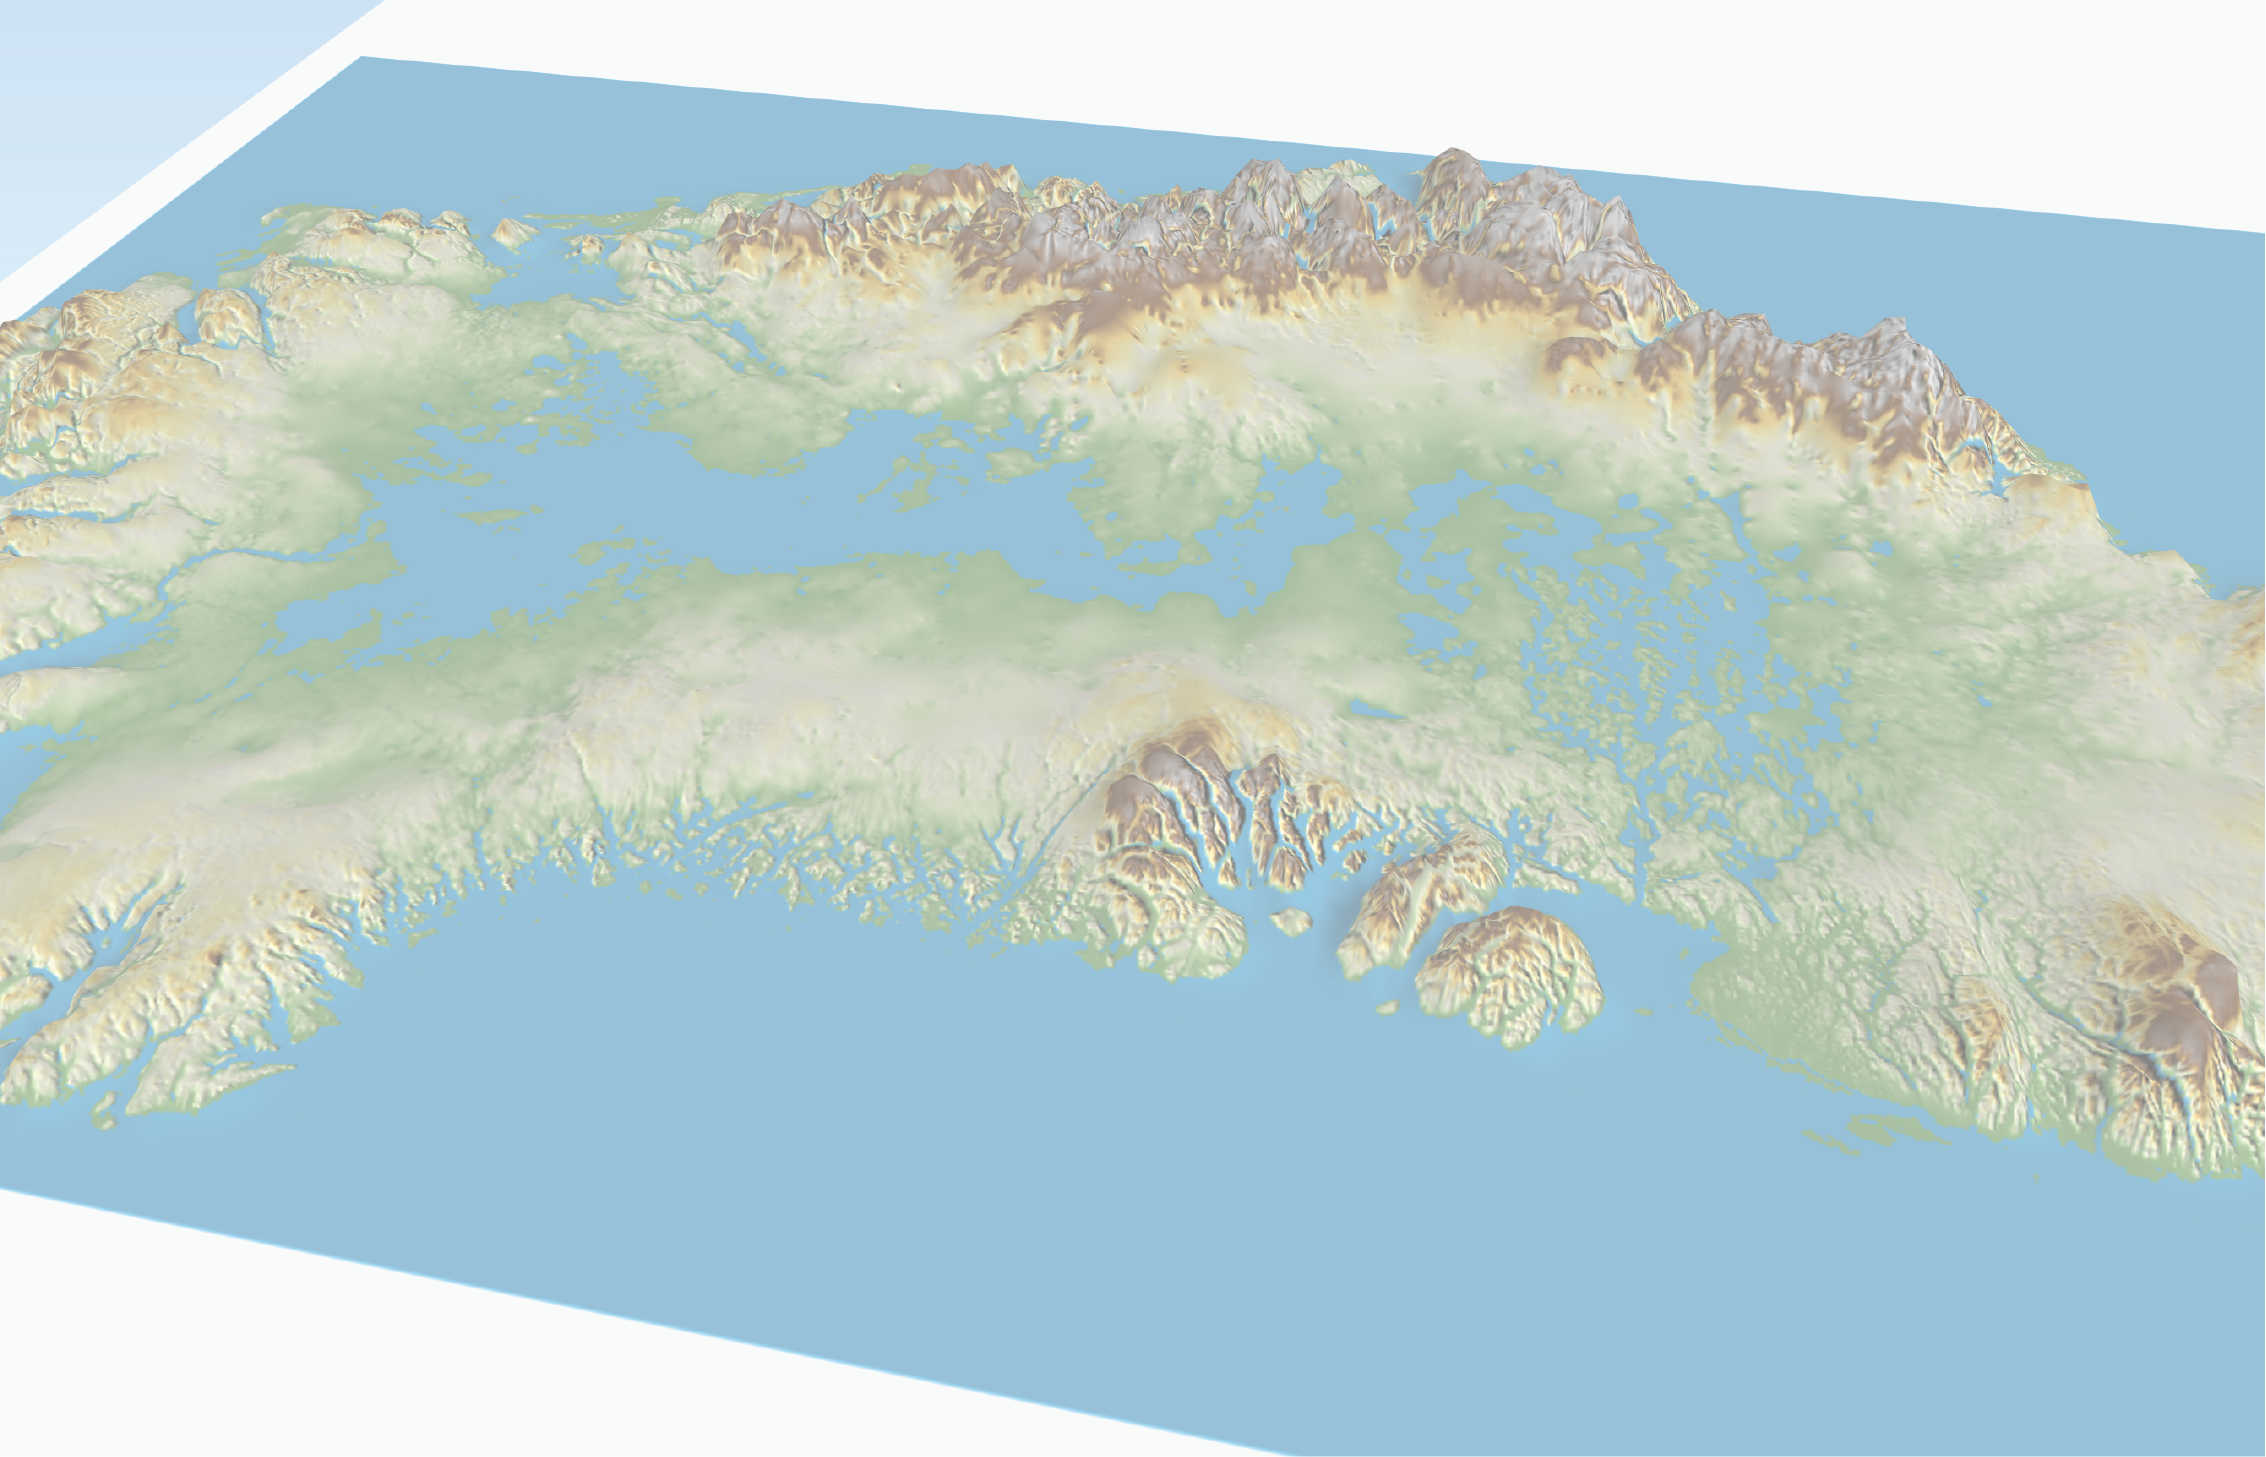
\includegraphics[height=\paperheight,width=\paperwidth]{gris-green-collage-clean-50op}};}
} 

\begin{frame}
  \frametitle{Main Findings}
  \begin{transbox}[0.5]
  \alert{$\Rightarrow$} Greenland could lose
  \begin{itemize}
    \item  5--19\,cm SLE (RCP 2.6), 8--23\,cm SLE (RCP 4.5), and 14--34\,cm SLE (RCP 8.5) by 2100
    \item  11--37\,cm SLE (RCP 2.6), 20--57\,cm SLE (RCP 4.5), and 52--156\,cm SLE (RCP 8.5) by 2200
  \end{itemize}
  \alert{$\Rightarrow$} Outlet glaciers will contribute
  \begin{itemize}
  \item 19--40\% of the total mass loss
  \end{itemize}
\end{transbox}
\end{frame}

\begin{frame}
  \frametitle{Main Findings}
  \begin{transbox}[0.5]
    \begin{itemize}
    \item We have performed the first millennium scale projections with an \textbf{outlet glacier-resolving} ice sheet model 
    \item Greenland will very likely become ice free in a millennium if we stay on an RCP 8.5 path
      \item better characterization of basal and surface processes are needed
    \end{itemize}
  \end{transbox}[0]
  \note[item]{In summary, Greenland will very likely become ice free within a millennium }
  \note[item]{if we keep following the RCP 8.5 scenario}
\end{frame}

\setbeamertemplate{background canvas}
  {
     \tikz{\node[inner sep=0pt,opacity=1] {\includegraphics[height=\paperheight,width=\paperwidth]{gris-green-collage-all}};}
} 


\begin{frame}[plain]
\end{frame}

\end{document}

